\documentclass[11pt]{article}
\usepackage[review]{acl}
\usepackage{multicol}
\usepackage{multirow}
\usepackage{soundver}
\usepackage{pgfplots}
\pgfplotsset{compat=1.17}
\usetikzlibrary{arrows.meta}
% generated by make_numbers.py (v4.1) -- do not edit
\newcommand{\ablDelAcc}{50.1}
\newcommand{\ablDelN}{3}
\newcommand{\ablDelRec}{0.34}
\newcommand{\ablDelRecMax}{0.35}
\newcommand{\ablDelRecMin}{0.33}
\newcommand{\ablGoldCatchIE}{52.0}
\newcommand{\ablGoldCatchSQL}{36.5}
\newcommand{\ablGoldClaimIE}{3.05}
\newcommand{\ablGoldClaimSQL}{5.19}
\newcommand{\ablGoldRatioIE}{0.3}
\newcommand{\ablGoldRatioSQL}{2.6}
\newcommand{\ablGoldTestIE}{0.99}
\newcommand{\ablGoldTestSQL}{13.38}
\newcommand{\ablGptCatchIE}{23.3}
\newcommand{\ablGptCatchSQL}{15.8}
\newcommand{\ablGptClaimIE}{4.13}
\newcommand{\ablGptClaimSQL}{3.41}
\newcommand{\ablGptTestIE}{1.19}
\newcommand{\ablGptTestSQL}{0.62}
\newcommand{\ablMainCatchIE}{52.0}
\newcommand{\ablMainCatchSQL}{23.1}
\newcommand{\ablMainClaimIE}{3.89}
\newcommand{\ablMainClaimSQL}{4.95}
\newcommand{\ablMainTestIE}{0.99}
\newcommand{\ablMainTestSQL}{1.61}
\newcommand{\ablOpusCatchIE}{50.2}
\newcommand{\ablOpusCatchSQL}{20.9}
\newcommand{\ablOpusClaimIE}{2.68}
\newcommand{\ablOpusClaimSQL}{2.42}
\newcommand{\ablOpusTestIE}{0.41}
\newcommand{\ablOpusTestSQL}{0.22}
\newcommand{\ablSingleCatchIE}{52.0}
\newcommand{\ablSingleCatchSQL}{23.1}
\newcommand{\ablSingleClaimIE}{3.05}
\newcommand{\ablSingleClaimSQL}{3.66}
\newcommand{\ablSingleTestIE}{0.99}
\newcommand{\ablSingleTestSQL}{1.61}
\newcommand{\advABmax}{85}
\newcommand{\advABmin}{78}
\newcommand{\advClPoorMax}{4}
\newcommand{\advClRichMax}{29}
\newcommand{\advClRichMin}{28}
\newcommand{\advGoldRejA}{86}
\newcommand{\advGoldRejB}{81}
\newcommand{\advMiscNCert}{1{,}659}
\newcommand{\advMiscNFone}{612}
\newcommand{\advMiscNNone}{5{,}453}
\newcommand{\advMiscNOracle}{222}
\newcommand{\advMiscPrecCert}{26}
\newcommand{\advMiscPrecFone}{8}
\newcommand{\advMiscPrecNone}{15}
\newcommand{\advMiscPrecOracle}{100}
\newcommand{\advMiscTitleCert}{58}
\newcommand{\advMiscTitleFone}{0}
\newcommand{\advMiscTitleNone}{41}
\newcommand{\advMiscTitleOracle}{88}
\newcommand{\boundBFC}{1.64}
\newcommand{\boundBFewnerd}{4.25}
\newcommand{\boundBIE}{3.89}
\newcommand{\boundBMath}{0.60}
\newcommand{\boundBMorph}{1.64}
\newcommand{\boundBSQL}{1.91}
\newcommand{\boundUApvFC}{2.17}
\newcommand{\boundUApvFewnerd}{0.41}
\newcommand{\boundUApvIE}{20.64}
\newcommand{\boundUApvMath}{2.55}
\newcommand{\boundUApvMorph}{0.41}
\newcommand{\boundUApvSQL}{17.78}
\newcommand{\boundUCertFC}{1.64}
\newcommand{\boundUCertFewnerd}{4.25}
\newcommand{\boundUCertIE}{3.89}
\newcommand{\boundUCertMath}{0.60}
\newcommand{\boundUCertMorph}{1.64}
\newcommand{\boundUCertSQL}{1.91}
\newcommand{\boundUFoneFC}{2.17}
\newcommand{\boundUFoneFewnerd}{1.51}
\newcommand{\boundUFoneIE}{20.53}
\newcommand{\boundUFoneMath}{0.60}
\newcommand{\boundUFoneMorph}{0.60}
\newcommand{\boundUFoneSQL}{3.77}
\newcommand{\boundUGroupFC}{0.93}
\newcommand{\boundUGroupFewnerd}{2.30}
\newcommand{\boundUGroupIE}{3.41}
\newcommand{\boundUGroupMath}{0.60}
\newcommand{\boundUGroupMorph}{0.60}
\newcommand{\boundUGroupSQL}{1.37}
\newcommand{\boundUHwFC}{1.08}
\newcommand{\boundUHwFewnerd}{0.93}
\newcommand{\boundUHwIE}{0.93}
\newcommand{\boundUHwMath}{48.91}
\newcommand{\boundUHwMorph}{31.35}
\newcommand{\boundUHwSQL}{0.77}
\newcommand{\bsDelMax}{0}
\newcommand{\bsRuns}{12}
\newcommand{\bsWorstMax}{18}
\newcommand{\budgetFC}{2}
\newcommand{\budgetFewnerd}{5}
\newcommand{\budgetIE}{5}
\newcommand{\budgetMath}{1}
\newcommand{\budgetMorph}{2}
\newcommand{\budgetSQL}{2}
\newcommand{\candFC}{45}
\newcommand{\candFewnerd}{73}
\newcommand{\candIE}{68}
\newcommand{\candMath}{107}
\newcommand{\candMorph}{49}
\newcommand{\candSQL}{134}
\newcommand{\candTotal}{476}
\newcommand{\catchApvFC}{76.8}
\newcommand{\catchApvFewnerd}{0.0}
\newcommand{\catchApvIE}{64.1}
\newcommand{\catchApvMath}{11.3}
\newcommand{\catchApvMorph}{0.0}
\newcommand{\catchApvSQL}{38.3}
\newcommand{\catchCertFC}{71.7}
\newcommand{\catchCertFewnerd}{28.2}
\newcommand{\catchCertIE}{52.5}
\newcommand{\catchCertMath}{9.7}
\newcommand{\catchCertMorph}{2.8}
\newcommand{\catchCertSQL}{20.4}
\newcommand{\catchFoneFC}{76.8}
\newcommand{\catchFoneFewnerd}{27.0}
\newcommand{\catchFoneIE}{64.0}
\newcommand{\catchFoneMath}{9.5}
\newcommand{\catchFoneMorph}{2.8}
\newcommand{\catchFoneSQL}{23.0}
\newcommand{\catchGroupFC}{71.4}
\newcommand{\catchGroupFewnerd}{27.2}
\newcommand{\catchGroupIE}{51.8}
\newcommand{\catchGroupMath}{9.5}
\newcommand{\catchGroupMorph}{2.4}
\newcommand{\catchGroupSQL}{0.9}
\newcommand{\catchHwFC}{70.2}
\newcommand{\catchHwFewnerd}{14.5}
\newcommand{\catchHwIE}{13.4}
\newcommand{\catchHwMath}{35.2}
\newcommand{\catchHwMorph}{24.3}
\newcommand{\catchHwSQL}{13.6}
\newcommand{\catchStrongIE}{40.7}
\newcommand{\catchStrongMorph}{0.4}
\newcommand{\ciCovSQLHi}{79}
\newcommand{\ciCovSQLLo}{66}
\newcommand{\ciDelFoneIEHi}{75}
\newcommand{\ciDelFoneIELo}{62}
\newcommand{\covCertFC}{100}
\newcommand{\covCertFewnerd}{100}
\newcommand{\covCertIE}{100}
\newcommand{\covCertMath}{93}
\newcommand{\covCertMorph}{100}
\newcommand{\covCertSQL}{73}
\newcommand{\coverageApvFC}{100}
\newcommand{\coverageApvFewnerd}{100}
\newcommand{\coverageApvIE}{100}
\newcommand{\coverageApvMath}{98}
\newcommand{\coverageApvMorph}{100}
\newcommand{\coverageApvSQL}{96}
\newcommand{\coverageCertFC}{100}
\newcommand{\coverageCertFewnerd}{100}
\newcommand{\coverageCertIE}{100}
\newcommand{\coverageCertMath}{93}
\newcommand{\coverageCertMorph}{100}
\newcommand{\coverageCertSQL}{73}
\newcommand{\coverageFoneFC}{100}
\newcommand{\coverageFoneFewnerd}{100}
\newcommand{\coverageFoneIE}{100}
\newcommand{\coverageFoneMath}{100}
\newcommand{\coverageFoneMorph}{100}
\newcommand{\coverageFoneSQL}{86}
\newcommand{\coverageFonecFC}{100}
\newcommand{\coverageFonecFewnerd}{99}
\newcommand{\coverageFonecIE}{100}
\newcommand{\coverageFonecMath}{100}
\newcommand{\coverageFonecMorph}{100}
\newcommand{\coverageFonecSQL}{77}
\newcommand{\coverageGroupFC}{100}
\newcommand{\coverageGroupFewnerd}{98}
\newcommand{\coverageGroupIE}{98}
\newcommand{\coverageGroupMath}{98}
\newcommand{\coverageGroupMorph}{100}
\newcommand{\coverageGroupSQL}{89}
\newcommand{\delRateApvFC}{0}
\newcommand{\delRateApvFewnerd}{0}
\newcommand{\delRateApvIE}{69}
\newcommand{\delRateApvMath}{0}
\newcommand{\delRateApvMorph}{0}
\newcommand{\delRateApvSQL}{3}
\newcommand{\delRateCertFC}{0}
\newcommand{\delRateCertFewnerd}{0}
\newcommand{\delRateCertIE}{0}
\newcommand{\delRateCertMath}{0}
\newcommand{\delRateCertMorph}{0}
\newcommand{\delRateCertSQL}{0}
\newcommand{\delRateFoneFC}{0}
\newcommand{\delRateFoneFewnerd}{0}
\newcommand{\delRateFoneIE}{69}
\newcommand{\delRateFoneMath}{0}
\newcommand{\delRateFoneMaxOther}{0.5}
\newcommand{\delRateFoneMorph}{0.5}
\newcommand{\delRateFoneSQL}{0}
\newcommand{\delRateFonecFC}{0}
\newcommand{\delRateFonecFewnerd}{0}
\newcommand{\delRateFonecIE}{0}
\newcommand{\delRateFonecMath}{0}
\newcommand{\delRateFonecMorph}{0}
\newcommand{\delRateFonecSQL}{0}
\newcommand{\delRateGroupFC}{0}
\newcommand{\delRateGroupFewnerd}{0}
\newcommand{\delRateGroupIE}{0}
\newcommand{\delRateGroupMath}{0}
\newcommand{\delRateGroupMorph}{0}
\newcommand{\delRateGroupSQL}{0}
\newcommand{\devVsFoneHiIELlama}{$-$1.0}
\newcommand{\devVsFoneHiIEMini}{+0.0}
\newcommand{\devVsFoneHiIEQwen}{+1.2}
\newcommand{\devVsFoneIELlama}{$-$2.9}
\newcommand{\devVsFoneIEMini}{$-$1.0}
\newcommand{\devVsFoneIEQwen}{$-$0.1}
\newcommand{\devVsFoneLoIELlama}{$-$4.8}
\newcommand{\devVsFoneLoIEMini}{$-$2.1}
\newcommand{\devVsFoneLoIEQwen}{$-$1.4}
\newcommand{\dsAccCert}{48.0}
\newcommand{\dsAccFone}{50.4}
\newcommand{\dsAccSdCert}{1.5}
\newcommand{\dsAccSdFone}{1.0}
\newcommand{\dsBigAccCert}{52.6}
\newcommand{\dsBigAccFone}{52.1}
\newcommand{\dsBigElseCert}{25.5}
\newcommand{\dsBigElseFone}{6.9}
\newcommand{\dsBigRecCert}{0.39}
\newcommand{\dsBigRecFone}{0.10}
\newcommand{\dsElseCert}{17.6}
\newcommand{\dsElseFone}{5.6}
\newcommand{\dsElseSdCert}{0.0}
\newcommand{\dsElseSdFone}{0.6}
\newcommand{\dsMatchedAcc}{49.1}
\newcommand{\dsMatchedElse}{15.4}
\newcommand{\dsMatchedRec}{0.29}
\newcommand{\dsRecCert}{0.31}
\newcommand{\dsRecFone}{0.08}
\newcommand{\dsRecSdCert}{0.00}
\newcommand{\dsRecSdFone}{0.03}
\newcommand{\eDelApv}{71}
\newcommand{\eDelBudget}{0}
\newcommand{\eDelFone}{0}
\newcommand{\eDelGroup}{0}
\newcommand{\eDelOutlvl}{0}
\newcommand{\eNnew}{63}
\newcommand{\eOtherApv}{71.0}
\newcommand{\eOtherBudget}{2.2}
\newcommand{\eOtherFone}{29.5}
\newcommand{\eOtherGroup}{1.0}
\newcommand{\eOtherOutlvl}{7.6}
\newcommand{\eOtherPnineApv}{100}
\newcommand{\eOtherPnineBudget}{4}
\newcommand{\eOtherPnineFone}{40}
\newcommand{\eOtherPnineGroup}{2}
\newcommand{\eOtherPnineOutlvl}{10}
\newcommand{\figMechClip}{5}
\newcommand{\figMechDanger}{8}
\newcommand{\figMechDangerInj}{7}
\newcommand{\figMechN}{387}
\newcommand{\fnAccCert}{32.9}
\newcommand{\fnAccFone}{30.2}
\newcommand{\fnAccHw}{29.4}
\newcommand{\fnDiffFone}{+2.7 [+0.7, +4.7]}
\newcommand{\fnDiffHw}{+3.5 [+1.5, +5.6]}
\newcommand{\fnDiffNone}{+6.2 [+4.1, +8.6]}
\newcommand{\fnSeedCert}{31.6}
\newcommand{\fnSeedFone}{30.6}
\newcommand{\fnSeedN}{3}
\newcommand{\fnSeedSdCert}{1.6}
\newcommand{\fnSeedSdFone}{0.4}
\newcommand{\frAccBaseFCLlama}{39.5}
\newcommand{\frAccBaseFCMini}{92.5}
\newcommand{\frAccBaseFCQwen}{95.3}
\newcommand{\frAccBaseFewnerdLlama}{34.0}
\newcommand{\frAccBaseFewnerdMini}{24.0}
\newcommand{\frAccBaseFewnerdQwen}{32.8}
\newcommand{\frAccBaseIELlama}{38.7}
\newcommand{\frAccBaseIEMini}{36.3}
\newcommand{\frAccBaseIEQwen}{49.2}
\newcommand{\frAccBaseMathLlama}{95.3}
\newcommand{\frAccBaseMathMini}{92.3}
\newcommand{\frAccBaseMathQwen}{93.3}
\newcommand{\frAccBaseMorphLlama}{34.7}
\newcommand{\frAccBaseMorphMini}{39.7}
\newcommand{\frAccBaseMorphQwen}{39.7}
\newcommand{\frAccBaseSQLLlama}{69.3}
\newcommand{\frAccBaseSQLMini}{75.0}
\newcommand{\frAccBaseSQLQwen}{76.7}
\newcommand{\frAccCertFCLlama}{41.7}
\newcommand{\frAccCertFCMini}{92.8}
\newcommand{\frAccCertFCQwen}{95.3}
\newcommand{\frAccCertFewnerdLlama}{36.3}
\newcommand{\frAccCertFewnerdMini}{25.7}
\newcommand{\frAccCertFewnerdQwen}{34.6}
\newcommand{\frAccCertIELlama}{51.8}
\newcommand{\frAccCertIEMini}{41.7}
\newcommand{\frAccCertIEQwen}{53.1}
\newcommand{\frAccCertMathLlama}{95.6}
\newcommand{\frAccCertMathMini}{93.0}
\newcommand{\frAccCertMathQwen}{94.5}
\newcommand{\frAccCertMorphLlama}{34.8}
\newcommand{\frAccCertMorphMini}{39.7}
\newcommand{\frAccCertMorphQwen}{39.8}
\newcommand{\frAccCertSQLLlama}{74.3}
\newcommand{\frAccCertSQLMini}{76.0}
\newcommand{\frAccCertSQLQwen}{77.4}
\newcommand{\frAccFoneFCLlama}{42.0}
\newcommand{\frAccFoneFCMini}{92.8}
\newcommand{\frAccFoneFCQwen}{95.5}
\newcommand{\frAccFoneFewnerdLlama}{36.4}
\newcommand{\frAccFoneFewnerdMini}{25.7}
\newcommand{\frAccFoneFewnerdQwen}{34.6}
\newcommand{\frAccFoneIELlama}{54.2}
\newcommand{\frAccFoneIEMini}{42.0}
\newcommand{\frAccFoneIEQwen}{52.4}
\newcommand{\frAccFoneMathLlama}{95.6}
\newcommand{\frAccFoneMathMini}{93.0}
\newcommand{\frAccFoneMathQwen}{94.5}
\newcommand{\frAccFoneMorphLlama}{34.8}
\newcommand{\frAccFoneMorphMini}{39.7}
\newcommand{\frAccFoneMorphQwen}{39.8}
\newcommand{\frAccFoneSQLLlama}{74.6}
\newcommand{\frAccFoneSQLMini}{76.0}
\newcommand{\frAccFoneSQLQwen}{77.7}
\newcommand{\frAccHwFCLlama}{42.2}
\newcommand{\frAccHwFCMini}{92.5}
\newcommand{\frAccHwFCQwen}{95.3}
\newcommand{\frAccHwFewnerdLlama}{34.7}
\newcommand{\frAccHwFewnerdMini}{24.8}
\newcommand{\frAccHwFewnerdQwen}{33.9}
\newcommand{\frAccHwIELlama}{45.5}
\newcommand{\frAccHwIEMini}{36.3}
\newcommand{\frAccHwIEQwen}{49.5}
\newcommand{\frAccHwMathLlama}{95.3}
\newcommand{\frAccHwMathMini}{93.2}
\newcommand{\frAccHwMathQwen}{94.4}
\newcommand{\frAccHwMorphLlama}{33.0}
\newcommand{\frAccHwMorphMini}{38.4}
\newcommand{\frAccHwMorphQwen}{38.7}
\newcommand{\frAccHwSQLLlama}{74.0}
\newcommand{\frAccHwSQLMini}{76.0}
\newcommand{\frAccHwSQLQwen}{77.4}
\newcommand{\frDltApvFCLlama}{0.4}
\newcommand{\frDltApvFCMini}{0.0}
\newcommand{\frDltApvFCQwen}{0.2}
\newcommand{\frDltApvFewnerdLlama}{0.0}
\newcommand{\frDltApvFewnerdMini}{0.0}
\newcommand{\frDltApvFewnerdQwen}{0.0}
\newcommand{\frDltApvIELlama}{11.9}
\newcommand{\frDltApvIEMini}{7.3}
\newcommand{\frDltApvIEQwen}{5.1}
\newcommand{\frDltApvMathLlama}{0.5}
\newcommand{\frDltApvMathMini}{0.3}
\newcommand{\frDltApvMathQwen}{0.4}
\newcommand{\frDltApvMorphLlama}{0.0}
\newcommand{\frDltApvMorphMini}{0.0}
\newcommand{\frDltApvMorphQwen}{0.0}
\newcommand{\frDltApvSQLLlama}{8.2}
\newcommand{\frDltApvSQLMini}{9.7}
\newcommand{\frDltApvSQLQwen}{9.1}
\newcommand{\frDltCertFCLlama}{1.2}
\newcommand{\frDltCertFCMini}{0.4}
\newcommand{\frDltCertFCQwen}{0.5}
\newcommand{\frDltCertFewnerdLlama}{2.5}
\newcommand{\frDltCertFewnerdMini}{1.8}
\newcommand{\frDltCertFewnerdQwen}{1.1}
\newcommand{\frDltCertIELlama}{2.0}
\newcommand{\frDltCertIEMini}{0.7}
\newcommand{\frDltCertIEQwen}{1.1}
\newcommand{\frDltCertMathLlama}{0.3}
\newcommand{\frDltCertMathMini}{0.3}
\newcommand{\frDltCertMathQwen}{0.3}
\newcommand{\frDltCertMorphLlama}{0.0}
\newcommand{\frDltCertMorphMini}{0.0}
\newcommand{\frDltCertMorphQwen}{0.0}
\newcommand{\frDltCertSQLLlama}{0.6}
\newcommand{\frDltCertSQLMini}{1.2}
\newcommand{\frDltCertSQLQwen}{0.6}
\newcommand{\frDltFoneFCLlama}{0.4}
\newcommand{\frDltFoneFCMini}{0.0}
\newcommand{\frDltFoneFCQwen}{0.2}
\newcommand{\frDltFoneFewnerdLlama}{0.5}
\newcommand{\frDltFoneFewnerdMini}{0.0}
\newcommand{\frDltFoneFewnerdQwen}{0.0}
\newcommand{\frDltFoneIELlama}{11.9}
\newcommand{\frDltFoneIEMini}{7.3}
\newcommand{\frDltFoneIEQwen}{5.1}
\newcommand{\frDltFoneMathLlama}{0.0}
\newcommand{\frDltFoneMathMini}{0.0}
\newcommand{\frDltFoneMathQwen}{0.0}
\newcommand{\frDltFoneMorphLlama}{0.0}
\newcommand{\frDltFoneMorphMini}{0.0}
\newcommand{\frDltFoneMorphQwen}{0.0}
\newcommand{\frDltFoneSQLLlama}{1.4}
\newcommand{\frDltFoneSQLMini}{1.6}
\newcommand{\frDltFoneSQLQwen}{1.0}
\newcommand{\frGainFCLlama}{$-$0.5}
\newcommand{\frGainFCMini}{+0.3}
\newcommand{\frGainFCQwen}{+0.0}
\newcommand{\frGainFewnerdLlama}{+1.6}
\newcommand{\frGainFewnerdMini}{+0.9}
\newcommand{\frGainFewnerdQwen}{+0.7}
\newcommand{\frGainHiFCLlama}{+0.0}
\newcommand{\frGainHiFCMini}{+0.8}
\newcommand{\frGainHiFCQwen}{+0.0}
\newcommand{\frGainHiFewnerdLlama}{+2.7}
\newcommand{\frGainHiFewnerdMini}{+1.7}
\newcommand{\frGainHiFewnerdQwen}{+1.6}
\newcommand{\frGainHiIELlama}{+8.9}
\newcommand{\frGainHiIEMini}{+8.0}
\newcommand{\frGainHiIEQwen}{+5.7}
\newcommand{\frGainHiMathLlama}{+1.0}
\newcommand{\frGainHiMathMini}{+1.3}
\newcommand{\frGainHiMathQwen}{+1.6}
\newcommand{\frGainHiMorphLlama}{+3.7}
\newcommand{\frGainHiMorphMini}{+2.9}
\newcommand{\frGainHiMorphQwen}{+3.1}
\newcommand{\frGainHiSQLLlama}{+1.0}
\newcommand{\frGainHiSQLMini}{+0.0}
\newcommand{\frGainHiSQLQwen}{+0.0}
\newcommand{\frGainIELlama}{+6.2}
\newcommand{\frGainIEMini}{+5.4}
\newcommand{\frGainIEQwen}{+3.6}
\newcommand{\frGainLoFCLlama}{$-$1.1}
\newcommand{\frGainLoFCMini}{+0.0}
\newcommand{\frGainLoFCQwen}{+0.0}
\newcommand{\frGainLoFewnerdLlama}{+0.6}
\newcommand{\frGainLoFewnerdMini}{+0.3}
\newcommand{\frGainLoFewnerdQwen}{+0.0}
\newcommand{\frGainLoIELlama}{+3.8}
\newcommand{\frGainLoIEMini}{+3.0}
\newcommand{\frGainLoIEQwen}{+1.7}
\newcommand{\frGainLoMathLlama}{$-$0.2}
\newcommand{\frGainLoMathMini}{$-$1.8}
\newcommand{\frGainLoMathQwen}{$-$1.5}
\newcommand{\frGainLoMorphLlama}{$-$0.1}
\newcommand{\frGainLoMorphMini}{$-$0.2}
\newcommand{\frGainLoMorphQwen}{$-$0.7}
\newcommand{\frGainLoSQLLlama}{+0.0}
\newcommand{\frGainLoSQLMini}{+0.0}
\newcommand{\frGainLoSQLQwen}{+0.0}
\newcommand{\frGainMathLlama}{+0.3}
\newcommand{\frGainMathMini}{$-$0.2}
\newcommand{\frGainMathQwen}{+0.0}
\newcommand{\frGainMorphLlama}{+1.7}
\newcommand{\frGainMorphMini}{+1.3}
\newcommand{\frGainMorphQwen}{+1.1}
\newcommand{\frGainSQLLlama}{+0.3}
\newcommand{\frGainSQLMini}{+0.0}
\newcommand{\frGainSQLQwen}{+0.0}
\newcommand{\frLostCertFC}{8/1407}
\newcommand{\frLostCertFewnerd}{13/776}
\newcommand{\frLostCertIE}{6/516}
\newcommand{\frLostCertMath}{3/877}
\newcommand{\frLostCertMorph}{0/452}
\newcommand{\frLostCertSQL}{3/754}
\newcommand{\frLostFoneFC}{2/1407}
\newcommand{\frLostFoneFewnerd}{1/776}
\newcommand{\frLostFoneIE}{42/516}
\newcommand{\frLostFoneMath}{0/877}
\newcommand{\frLostFoneMorph}{0/452}
\newcommand{\frLostFoneSQL}{7/754}
\newcommand{\frLostHwFC}{0/1407}
\newcommand{\frLostHwFewnerd}{0/776}
\newcommand{\frLostHwIE}{0/516}
\newcommand{\frLostHwMath}{1/877}
\newcommand{\frLostHwMorph}{80/452}
\newcommand{\frLostHwSQL}{0/754}
\newcommand{\frPrecCertFC}{0.928}
\newcommand{\frPrecCertFewnerd}{0.370}
\newcommand{\frPrecCertIE}{0.579}
\newcommand{\frPrecCertMath}{0.944}
\newcommand{\frPrecCertMorph}{0.381}
\newcommand{\frPrecCertSQL}{0.780}
\newcommand{\frPrecFoneFC}{0.944}
\newcommand{\frPrecFoneFewnerd}{0.371}
\newcommand{\frPrecFoneIE}{0.624}
\newcommand{\frPrecFoneMath}{0.945}
\newcommand{\frPrecFoneMorph}{0.381}
\newcommand{\frPrecFoneSQL}{0.784}
\newcommand{\frPrecHwFC}{0.924}
\newcommand{\frPrecHwFewnerd}{0.333}
\newcommand{\frPrecHwIE}{0.442}
\newcommand{\frPrecHwMath}{0.948}
\newcommand{\frPrecHwMorph}{0.411}
\newcommand{\frPrecHwSQL}{0.770}
\newcommand{\frRecCertFC}{0.996}
\newcommand{\frRecCertFewnerd}{0.983}
\newcommand{\frRecCertIE}{0.987}
\newcommand{\frRecCertMath}{0.996}
\newcommand{\frRecCertMorph}{1.000}
\newcommand{\frRecCertSQL}{0.995}
\newcommand{\frRecFoneFC}{0.999}
\newcommand{\frRecFoneFewnerd}{0.999}
\newcommand{\frRecFoneIE}{0.938}
\newcommand{\frRecFoneMath}{1.000}
\newcommand{\frRecFoneMorph}{1.000}
\newcommand{\frRecFoneSQL}{0.988}
\newcommand{\frRecHwFC}{1.000}
\newcommand{\frRecHwFewnerd}{0.999}
\newcommand{\frRecHwIE}{0.999}
\newcommand{\frRecHwMath}{0.926}
\newcommand{\frRecHwMorph}{0.864}
\newcommand{\frRecHwSQL}{0.997}
\newcommand{\frSubCertFCArg}{0/500}
\newcommand{\frSubCertFCArgs}{0/597}
\newcommand{\frSubCertFCBoolArg}{0/16}
\newcommand{\frSubCertFCEnumParam}{0/15}
\newcommand{\frSubCertFCMultiFunctionChoice}{3/367}
\newcommand{\frSubCertFCNumericArg}{0/539}
\newcommand{\frSubCertFCPlusArgs}{8/310}
\newcommand{\frSubCertFCStructuredArg}{0/144}
\newcommand{\frSubCertFewnerdHasArt}{0/55}
\newcommand{\frSubCertFewnerdHasBuilding}{0/54}
\newcommand{\frSubCertFewnerdHasEvent}{1/36}
\newcommand{\frSubCertFewnerdHasLocation}{5/216}
\newcommand{\frSubCertFewnerdHasOrganization}{4/175}
\newcommand{\frSubCertFewnerdHasOther}{3/73}
\newcommand{\frSubCertFewnerdHasPerson}{0/212}
\newcommand{\frSubCertFewnerdHasProduct}{1/42}
\newcommand{\frSubCertFewnerdNoEntities}{0/190}
\newcommand{\frSubCertFewnerdPlusEntities}{5/88}
\newcommand{\frSubCertIEEntityPlusTokens}{4/31}
\newcommand{\frSubCertIEEntityWithLowercaseToken}{1/6}
\newcommand{\frSubCertIEHasElseType}{1/44}
\newcommand{\frSubCertIENoEntities}{0/135}
\newcommand{\frSubCertIEPlain}{0/286}
\newcommand{\frSubCertIEPlusEntities}{5/49}
\newcommand{\frSubCertMathAnswerGe}{0/85}
\newcommand{\frSubCertMathPlusSteps}{3/156}
\newcommand{\frSubCertMathSteps}{0/275}
\newcommand{\frSubCertMorphCanonicalDiffersFromSurface}{0/80}
\newcommand{\frSubCertMorphMorphemes}{0/24}
\newcommand{\frSubCertSQLAggregate}{3/399}
\newcommand{\frSubCertSQLGroupBy}{0/171}
\newcommand{\frSubCertSQLHaving}{0/46}
\newcommand{\frSubCertSQLJoin}{0/253}
\newcommand{\frSubCertSQLLike}{0/6}
\newcommand{\frSubCertSQLNestedOrSetop}{0/106}
\newcommand{\frSubCertSQLOrderBy}{0/161}
\newcommand{\frSubCertSQLSimple}{3/295}
\newcommand{\frSubFoneFCArg}{0/500}
\newcommand{\frSubFoneFCArgs}{0/597}
\newcommand{\frSubFoneFCBoolArg}{0/16}
\newcommand{\frSubFoneFCEnumParam}{0/15}
\newcommand{\frSubFoneFCMultiFunctionChoice}{0/367}
\newcommand{\frSubFoneFCNumericArg}{0/539}
\newcommand{\frSubFoneFCPlusArgs}{2/310}
\newcommand{\frSubFoneFCStructuredArg}{0/144}
\newcommand{\frSubFoneFewnerdHasArt}{0/55}
\newcommand{\frSubFoneFewnerdHasBuilding}{0/54}
\newcommand{\frSubFoneFewnerdHasEvent}{0/36}
\newcommand{\frSubFoneFewnerdHasLocation}{0/216}
\newcommand{\frSubFoneFewnerdHasOrganization}{0/175}
\newcommand{\frSubFoneFewnerdHasOther}{0/73}
\newcommand{\frSubFoneFewnerdHasPerson}{0/212}
\newcommand{\frSubFoneFewnerdHasProduct}{1/42}
\newcommand{\frSubFoneFewnerdNoEntities}{0/190}
\newcommand{\frSubFoneFewnerdPlusEntities}{0/88}
\newcommand{\frSubFoneIEEntityPlusTokens}{9/31}
\newcommand{\frSubFoneIEEntityWithLowercaseToken}{2/6}
\newcommand{\frSubFoneIEHasElseType}{37/44}
\newcommand{\frSubFoneIENoEntities}{0/135}
\newcommand{\frSubFoneIEPlain}{0/286}
\newcommand{\frSubFoneIEPlusEntities}{19/49}
\newcommand{\frSubFoneMathAnswerGe}{0/85}
\newcommand{\frSubFoneMathPlusSteps}{0/156}
\newcommand{\frSubFoneMathSteps}{0/275}
\newcommand{\frSubFoneMorphCanonicalDiffersFromSurface}{0/80}
\newcommand{\frSubFoneMorphMorphemes}{0/24}
\newcommand{\frSubFoneSQLAggregate}{4/399}
\newcommand{\frSubFoneSQLGroupBy}{0/171}
\newcommand{\frSubFoneSQLHaving}{0/46}
\newcommand{\frSubFoneSQLJoin}{3/253}
\newcommand{\frSubFoneSQLLike}{0/6}
\newcommand{\frSubFoneSQLNestedOrSetop}{3/106}
\newcommand{\frSubFoneSQLOrderBy}{3/161}
\newcommand{\frSubFoneSQLSimple}{1/295}
\newcommand{\frSubHwFCArg}{0/500}
\newcommand{\frSubHwFCArgs}{0/597}
\newcommand{\frSubHwFCBoolArg}{0/16}
\newcommand{\frSubHwFCEnumParam}{0/15}
\newcommand{\frSubHwFCMultiFunctionChoice}{0/367}
\newcommand{\frSubHwFCNumericArg}{0/539}
\newcommand{\frSubHwFCPlusArgs}{0/310}
\newcommand{\frSubHwFCStructuredArg}{0/144}
\newcommand{\frSubHwFewnerdHasArt}{0/55}
\newcommand{\frSubHwFewnerdHasBuilding}{0/54}
\newcommand{\frSubHwFewnerdHasEvent}{0/36}
\newcommand{\frSubHwFewnerdHasLocation}{0/216}
\newcommand{\frSubHwFewnerdHasOrganization}{0/175}
\newcommand{\frSubHwFewnerdHasOther}{0/73}
\newcommand{\frSubHwFewnerdHasPerson}{0/212}
\newcommand{\frSubHwFewnerdHasProduct}{0/42}
\newcommand{\frSubHwFewnerdNoEntities}{0/190}
\newcommand{\frSubHwFewnerdPlusEntities}{0/88}
\newcommand{\frSubHwIEEntityPlusTokens}{0/31}
\newcommand{\frSubHwIEEntityWithLowercaseToken}{0/6}
\newcommand{\frSubHwIEHasElseType}{0/44}
\newcommand{\frSubHwIENoEntities}{0/135}
\newcommand{\frSubHwIEPlain}{0/286}
\newcommand{\frSubHwIEPlusEntities}{0/49}
\newcommand{\frSubHwMathAnswerGe}{0/85}
\newcommand{\frSubHwMathPlusSteps}{1/156}
\newcommand{\frSubHwMathSteps}{0/275}
\newcommand{\frSubHwMorphCanonicalDiffersFromSurface}{80/80}
\newcommand{\frSubHwMorphMorphemes}{7/24}
\newcommand{\frSubHwSQLAggregate}{0/399}
\newcommand{\frSubHwSQLGroupBy}{0/171}
\newcommand{\frSubHwSQLHaving}{0/46}
\newcommand{\frSubHwSQLJoin}{0/253}
\newcommand{\frSubHwSQLLike}{0/6}
\newcommand{\frSubHwSQLNestedOrSetop}{0/106}
\newcommand{\frSubHwSQLOrderBy}{0/161}
\newcommand{\frSubHwSQLSimple}{0/295}
\newcommand{\frSubPctCertFCArg}{0}
\newcommand{\frSubPctCertFCArgs}{0}
\newcommand{\frSubPctCertFCBoolArg}{0}
\newcommand{\frSubPctCertFCEnumParam}{0}
\newcommand{\frSubPctCertFCMultiFunctionChoice}{1}
\newcommand{\frSubPctCertFCNumericArg}{0}
\newcommand{\frSubPctCertFCPlusArgs}{3}
\newcommand{\frSubPctCertFCStructuredArg}{0}
\newcommand{\frSubPctCertFewnerdHasArt}{0}
\newcommand{\frSubPctCertFewnerdHasBuilding}{0}
\newcommand{\frSubPctCertFewnerdHasEvent}{3}
\newcommand{\frSubPctCertFewnerdHasLocation}{2}
\newcommand{\frSubPctCertFewnerdHasOrganization}{2}
\newcommand{\frSubPctCertFewnerdHasOther}{4}
\newcommand{\frSubPctCertFewnerdHasPerson}{0}
\newcommand{\frSubPctCertFewnerdHasProduct}{2}
\newcommand{\frSubPctCertFewnerdNoEntities}{0}
\newcommand{\frSubPctCertFewnerdPlusEntities}{6}
\newcommand{\frSubPctCertIEEntityPlusTokens}{13}
\newcommand{\frSubPctCertIEEntityWithLowercaseToken}{17}
\newcommand{\frSubPctCertIEHasElseType}{2}
\newcommand{\frSubPctCertIENoEntities}{0}
\newcommand{\frSubPctCertIEPlain}{0}
\newcommand{\frSubPctCertIEPlusEntities}{10}
\newcommand{\frSubPctCertMathAnswerGe}{0}
\newcommand{\frSubPctCertMathPlusSteps}{2}
\newcommand{\frSubPctCertMathSteps}{0}
\newcommand{\frSubPctCertMorphCanonicalDiffersFromSurface}{0}
\newcommand{\frSubPctCertMorphMorphemes}{0}
\newcommand{\frSubPctCertSQLAggregate}{1}
\newcommand{\frSubPctCertSQLGroupBy}{0}
\newcommand{\frSubPctCertSQLHaving}{0}
\newcommand{\frSubPctCertSQLJoin}{0}
\newcommand{\frSubPctCertSQLLike}{0}
\newcommand{\frSubPctCertSQLNestedOrSetop}{0}
\newcommand{\frSubPctCertSQLOrderBy}{0}
\newcommand{\frSubPctCertSQLSimple}{1}
\newcommand{\frSubPctFoneFCArg}{0}
\newcommand{\frSubPctFoneFCArgs}{0}
\newcommand{\frSubPctFoneFCBoolArg}{0}
\newcommand{\frSubPctFoneFCEnumParam}{0}
\newcommand{\frSubPctFoneFCMultiFunctionChoice}{0}
\newcommand{\frSubPctFoneFCNumericArg}{0}
\newcommand{\frSubPctFoneFCPlusArgs}{1}
\newcommand{\frSubPctFoneFCStructuredArg}{0}
\newcommand{\frSubPctFoneFewnerdHasArt}{0}
\newcommand{\frSubPctFoneFewnerdHasBuilding}{0}
\newcommand{\frSubPctFoneFewnerdHasEvent}{0}
\newcommand{\frSubPctFoneFewnerdHasLocation}{0}
\newcommand{\frSubPctFoneFewnerdHasOrganization}{0}
\newcommand{\frSubPctFoneFewnerdHasOther}{0}
\newcommand{\frSubPctFoneFewnerdHasPerson}{0}
\newcommand{\frSubPctFoneFewnerdHasProduct}{2}
\newcommand{\frSubPctFoneFewnerdNoEntities}{0}
\newcommand{\frSubPctFoneFewnerdPlusEntities}{0}
\newcommand{\frSubPctFoneIEEntityPlusTokens}{29}
\newcommand{\frSubPctFoneIEEntityWithLowercaseToken}{33}
\newcommand{\frSubPctFoneIEHasElseType}{84}
\newcommand{\frSubPctFoneIENoEntities}{0}
\newcommand{\frSubPctFoneIEPlain}{0}
\newcommand{\frSubPctFoneIEPlusEntities}{39}
\newcommand{\frSubPctFoneMathAnswerGe}{0}
\newcommand{\frSubPctFoneMathPlusSteps}{0}
\newcommand{\frSubPctFoneMathSteps}{0}
\newcommand{\frSubPctFoneMorphCanonicalDiffersFromSurface}{0}
\newcommand{\frSubPctFoneMorphMorphemes}{0}
\newcommand{\frSubPctFoneSQLAggregate}{1}
\newcommand{\frSubPctFoneSQLGroupBy}{0}
\newcommand{\frSubPctFoneSQLHaving}{0}
\newcommand{\frSubPctFoneSQLJoin}{1}
\newcommand{\frSubPctFoneSQLLike}{0}
\newcommand{\frSubPctFoneSQLNestedOrSetop}{3}
\newcommand{\frSubPctFoneSQLOrderBy}{2}
\newcommand{\frSubPctFoneSQLSimple}{0}
\newcommand{\frSubPctHwFCArg}{0}
\newcommand{\frSubPctHwFCArgs}{0}
\newcommand{\frSubPctHwFCBoolArg}{0}
\newcommand{\frSubPctHwFCEnumParam}{0}
\newcommand{\frSubPctHwFCMultiFunctionChoice}{0}
\newcommand{\frSubPctHwFCNumericArg}{0}
\newcommand{\frSubPctHwFCPlusArgs}{0}
\newcommand{\frSubPctHwFCStructuredArg}{0}
\newcommand{\frSubPctHwFewnerdHasArt}{0}
\newcommand{\frSubPctHwFewnerdHasBuilding}{0}
\newcommand{\frSubPctHwFewnerdHasEvent}{0}
\newcommand{\frSubPctHwFewnerdHasLocation}{0}
\newcommand{\frSubPctHwFewnerdHasOrganization}{0}
\newcommand{\frSubPctHwFewnerdHasOther}{0}
\newcommand{\frSubPctHwFewnerdHasPerson}{0}
\newcommand{\frSubPctHwFewnerdHasProduct}{0}
\newcommand{\frSubPctHwFewnerdNoEntities}{0}
\newcommand{\frSubPctHwFewnerdPlusEntities}{0}
\newcommand{\frSubPctHwIEEntityPlusTokens}{0}
\newcommand{\frSubPctHwIEEntityWithLowercaseToken}{0}
\newcommand{\frSubPctHwIEHasElseType}{0}
\newcommand{\frSubPctHwIENoEntities}{0}
\newcommand{\frSubPctHwIEPlain}{0}
\newcommand{\frSubPctHwIEPlusEntities}{0}
\newcommand{\frSubPctHwMathAnswerGe}{0}
\newcommand{\frSubPctHwMathPlusSteps}{1}
\newcommand{\frSubPctHwMathSteps}{0}
\newcommand{\frSubPctHwMorphCanonicalDiffersFromSurface}{100}
\newcommand{\frSubPctHwMorphMorphemes}{29}
\newcommand{\frSubPctHwSQLAggregate}{0}
\newcommand{\frSubPctHwSQLGroupBy}{0}
\newcommand{\frSubPctHwSQLHaving}{0}
\newcommand{\frSubPctHwSQLJoin}{0}
\newcommand{\frSubPctHwSQLLike}{0}
\newcommand{\frSubPctHwSQLNestedOrSetop}{0}
\newcommand{\frSubPctHwSQLOrderBy}{0}
\newcommand{\frSubPctHwSQLSimple}{0}
\newcommand{\frVsFoneFCLlama}{$-$0.3}
\newcommand{\frVsFoneFCMini}{+0.0}
\newcommand{\frVsFoneFCQwen}{$-$0.2}
\newcommand{\frVsFoneFewnerdLlama}{$-$0.2}
\newcommand{\frVsFoneFewnerdMini}{+0.0}
\newcommand{\frVsFoneFewnerdQwen}{+0.0}
\newcommand{\frVsFoneHiFCLlama}{+0.0}
\newcommand{\frVsFoneHiFCMini}{+0.0}
\newcommand{\frVsFoneHiFCQwen}{+0.0}
\newcommand{\frVsFoneHiFewnerdLlama}{+0.0}
\newcommand{\frVsFoneHiFewnerdMini}{+0.0}
\newcommand{\frVsFoneHiFewnerdQwen}{+0.5}
\newcommand{\frVsFoneHiIELlama}{+0.5}
\newcommand{\frVsFoneHiIEMini}{+1.4}
\newcommand{\frVsFoneHiIEQwen}{+1.7}
\newcommand{\frVsFoneHiMathLlama}{+0.0}
\newcommand{\frVsFoneHiMathMini}{+0.0}
\newcommand{\frVsFoneHiMathQwen}{+0.0}
\newcommand{\frVsFoneHiMorphLlama}{+0.0}
\newcommand{\frVsFoneHiMorphMini}{+0.0}
\newcommand{\frVsFoneHiMorphQwen}{+0.0}
\newcommand{\frVsFoneHiSQLLlama}{+0.0}
\newcommand{\frVsFoneHiSQLMini}{+0.0}
\newcommand{\frVsFoneHiSQLQwen}{+0.0}
\newcommand{\frVsFoneIELlama}{$-$2.5}
\newcommand{\frVsFoneIEMini}{$-$0.3}
\newcommand{\frVsFoneIEQwen}{+0.6}
\newcommand{\frVsFoneLoFCLlama}{$-$0.8}
\newcommand{\frVsFoneLoFCMini}{+0.0}
\newcommand{\frVsFoneLoFCQwen}{$-$0.5}
\newcommand{\frVsFoneLoFewnerdLlama}{$-$0.5}
\newcommand{\frVsFoneLoFewnerdMini}{+0.0}
\newcommand{\frVsFoneLoFewnerdQwen}{$-$0.5}
\newcommand{\frVsFoneLoIELlama}{$-$5.6}
\newcommand{\frVsFoneLoIEMini}{$-$2.0}
\newcommand{\frVsFoneLoIEQwen}{$-$0.1}
\newcommand{\frVsFoneLoMathLlama}{+0.0}
\newcommand{\frVsFoneLoMathMini}{+0.0}
\newcommand{\frVsFoneLoMathQwen}{+0.0}
\newcommand{\frVsFoneLoMorphLlama}{+0.0}
\newcommand{\frVsFoneLoMorphMini}{+0.0}
\newcommand{\frVsFoneLoMorphQwen}{+0.0}
\newcommand{\frVsFoneLoSQLLlama}{$-$1.0}
\newcommand{\frVsFoneLoSQLMini}{+0.0}
\newcommand{\frVsFoneLoSQLQwen}{$-$1.0}
\newcommand{\frVsFoneMathLlama}{+0.0}
\newcommand{\frVsFoneMathMini}{+0.0}
\newcommand{\frVsFoneMathQwen}{+0.0}
\newcommand{\frVsFoneMorphLlama}{+0.0}
\newcommand{\frVsFoneMorphMini}{+0.0}
\newcommand{\frVsFoneMorphQwen}{+0.0}
\newcommand{\frVsFoneSQLLlama}{$-$0.3}
\newcommand{\frVsFoneSQLMini}{+0.0}
\newcommand{\frVsFoneSQLQwen}{$-$0.3}
\newcommand{\gammaKApvFC}{12}
\newcommand{\gammaKApvFewnerd}{0}
\newcommand{\gammaKApvIE}{179}
\newcommand{\gammaKApvMath}{15}
\newcommand{\gammaKApvMorph}{0}
\newcommand{\gammaKApvSQL}{152}
\newcommand{\gammaKCertFC}{8}
\newcommand{\gammaKCertFewnerd}{29}
\newcommand{\gammaKCertIE}{26}
\newcommand{\gammaKCertMath}{1}
\newcommand{\gammaKCertMorph}{8}
\newcommand{\gammaKCertSQL}{10}
\newcommand{\gammaKFoneFC}{12}
\newcommand{\gammaKFoneFewnerd}{7}
\newcommand{\gammaKFoneIE}{178}
\newcommand{\gammaKFoneMath}{1}
\newcommand{\gammaKFoneMorph}{1}
\newcommand{\gammaKFoneSQL}{25}
\newcommand{\gammaKGroupFC}{3}
\newcommand{\gammaKGroupFewnerd}{13}
\newcommand{\gammaKGroupIE}{22}
\newcommand{\gammaKGroupMath}{1}
\newcommand{\gammaKGroupMorph}{1}
\newcommand{\gammaKGroupSQL}{6}
\newcommand{\gammaKHwFC}{4}
\newcommand{\gammaKHwFewnerd}{3}
\newcommand{\gammaKHwIE}{3}
\newcommand{\gammaKHwMath}{455}
\newcommand{\gammaKHwMorph}{282}
\newcommand{\gammaKHwSQL}{2}
\newcommand{\gammaKStrongIE}{5}
\newcommand{\gammaKStrongMorph}{0}
\newcommand{\groupsNFC}{10}
\newcommand{\groupsNFewnerd}{14}
\newcommand{\groupsNIE}{10}
\newcommand{\groupsNMath}{8}
\newcommand{\groupsNMorph}{11}
\newcommand{\groupsNSQL}{14}
\newcommand{\injDelBudget}{0}
\newcommand{\injDelFone}{99.5}
\newcommand{\injDelFoneSQL}{0}
\newcommand{\injDelFonec}{0}
\newcommand{\injDelGroup}{0}
\newcommand{\injGammaKFone}{349}
\newcommand{\injInConstrained}{0}
\newcommand{\injNFewnerd}{8}
\newcommand{\injNPicked}{4}
\newcommand{\injPicked}{building, event, other and product}
\newcommand{\injPrecPickedMax}{0.18}
\newcommand{\injPrecSQL}{0.65}
\newcommand{\injPrecUnpickedMin}{0.24}
\newcommand{\injTestGammaFone}{35.5}
\newcommand{\injThrPickedMin}{0.31}
\newcommand{\injWipedFone}{100}
\newcommand{\injWipedGroupFone}{building}
\newcommand{\labelFalseNeg}{10.4}
\newcommand{\labelFalsePos}{3.7}
\newcommand{\labelN}{18{,}346}
\newcommand{\nChecksApvFC}{7}
\newcommand{\nChecksApvFewnerd}{0}
\newcommand{\nChecksApvIE}{13}
\newcommand{\nChecksApvMath}{9}
\newcommand{\nChecksApvMorph}{0}
\newcommand{\nChecksApvSQL}{16}
\newcommand{\nChecksCertFC}{6}
\newcommand{\nChecksCertFewnerd}{20}
\newcommand{\nChecksCertIE}{18}
\newcommand{\nChecksCertMath}{7}
\newcommand{\nChecksCertMorph}{7}
\newcommand{\nChecksCertSQL}{6}
\newcommand{\nChecksFoneFC}{7}
\newcommand{\nChecksFoneFewnerd}{16}
\newcommand{\nChecksFoneIE}{12}
\newcommand{\nChecksFoneMath}{5}
\newcommand{\nChecksFoneMorph}{6}
\newcommand{\nChecksFoneSQL}{10}
\newcommand{\nChecksGroupFC}{6}
\newcommand{\nChecksGroupFewnerd}{18}
\newcommand{\nChecksGroupIE}{16}
\newcommand{\nChecksGroupMath}{6}
\newcommand{\nChecksGroupMorph}{6}
\newcommand{\nChecksGroupSQL}{7}
\newcommand{\nChecksHwFC}{6}
\newcommand{\nChecksHwFewnerd}{4}
\newcommand{\nChecksHwIE}{4}
\newcommand{\nChecksHwMath}{2}
\newcommand{\nChecksHwMorph}{2}
\newcommand{\nChecksHwSQL}{3}
\newcommand{\nDeletableFC}{0}
\newcommand{\nDeletableFewnerd}{4}
\newcommand{\nDeletableIE}{1}
\newcommand{\nDeletableMath}{0}
\newcommand{\nDeletableMorph}{2}
\newcommand{\nDeletableSQL}{0}
\newcommand{\nIsolatingIE}{1}
\newcommand{\nIsolatingOther}{0}
\newcommand{\nRepTotal}{1{,}200}
\newcommand{\precIEElse}{0.23}
\newcommand{\rdAvailIE}{138}
\newcommand{\rdCatchBudgetIE}{49.0}
\newcommand{\rdCatchBudgetInj}{26.9}
\newcommand{\rdCatchOutlvlIE}{49.5}
\newcommand{\rdCatchOutlvlInj}{27.2}
\newcommand{\rdDelAvailApvIE}{100}
\newcommand{\rdDelAvailBudgetIE}{0}
\newcommand{\rdDelAvailFoneIE}{100}
\newcommand{\rdDelAvailOutlvlIE}{0}
\newcommand{\rdDelNotApvIE}{0}
\newcommand{\rdDelNotBudgetIE}{0}
\newcommand{\rdDelNotFoneIE}{0}
\newcommand{\rdDelNotOutlvlIE}{0}
\newcommand{\rdDelOutlvlInj}{0}
\newcommand{\rdDelOutlvlMax}{0}
\newcommand{\rdNIE}{200}
\newcommand{\rdNTasksOutlvl}{7}
\newcommand{\resCatchApvFC}{74.9}
\newcommand{\resCatchApvFewnerd}{0.0}
\newcommand{\resCatchApvIE}{54.3}
\newcommand{\resCatchApvMath}{9.5}
\newcommand{\resCatchApvMorph}{0.0}
\newcommand{\resCatchApvSQL}{36.1}
\newcommand{\resCatchCertFC}{72.7}
\newcommand{\resCatchCertFewnerd}{27.0}
\newcommand{\resCatchCertIE}{49.0}
\newcommand{\resCatchCertMath}{9.0}
\newcommand{\resCatchCertMorph}{2.2}
\newcommand{\resCatchCertSQL}{18.0}
\newcommand{\resCatchFoneFC}{74.9}
\newcommand{\resCatchFoneFewnerd}{27.7}
\newcommand{\resCatchFoneIE}{58.2}
\newcommand{\resCatchFoneMath}{8.5}
\newcommand{\resCatchFoneMorph}{2.2}
\newcommand{\resCatchFoneSQL}{22.6}
\newcommand{\resCatchFonecFC}{72.1}
\newcommand{\resCatchFonecFewnerd}{26.7}
\newcommand{\resCatchFonecIE}{48.9}
\newcommand{\resCatchFonecMath}{8.5}
\newcommand{\resCatchFonecMorph}{2.0}
\newcommand{\resCatchFonecSQL}{18.0}
\newcommand{\resCatchGroupFC}{70.5}
\newcommand{\resCatchGroupFewnerd}{23.8}
\newcommand{\resCatchGroupIE}{45.5}
\newcommand{\resCatchGroupMath}{8.5}
\newcommand{\resCatchGroupMorph}{1.9}
\newcommand{\resCatchGroupSQL}{5.3}
\newcommand{\rlAccCert}{65.0$\pm$0.3}
\newcommand{\rlAccFone}{62.8$\pm$0.6}
\newcommand{\rlAccInit}{63.6}
\newcommand{\rlAccLabel}{64.0 / 67.9}
\newcommand{\rlElseBase}{2.9}
\newcommand{\rlElseCert}{26.5$\pm$6.0}
\newcommand{\rlElseFone}{6.4$\pm$4.6}
\newcommand{\rlElseInit}{25.5}
\newcommand{\rlElseLabel}{26.5 / 35.3}
\newcommand{\rlNCert}{4}
\newcommand{\rlNFone}{4}
\newcommand{\rlNInit}{1}
\newcommand{\rlNLabel}{2}
\newcommand{\rlRecBase}{0.11}
\newcommand{\rlRecCert}{0.40$\pm$0.08}
\newcommand{\rlRecFone}{0.11$\pm$0.04}
\newcommand{\rlRecInit}{0.37}
\newcommand{\rlRecLabel}{0.42 / 0.55}
\newcommand{\rlRecMaxCert}{0.49}
\newcommand{\rlRecMaxFone}{0.15}
\newcommand{\rlRecMaxInit}{0.37}
\newcommand{\rlRecMaxLabel}{0.55}
\newcommand{\rlRecMinCert}{0.32}
\newcommand{\rlRecMinFone}{0.08}
\newcommand{\rlRecMinInit}{0.37}
\newcommand{\rlRecMinLabel}{0.42}
\newcommand{\rtFoneNoGoldTakes}{yes}
\newcommand{\rtFreshHoldN}{3}
\newcommand{\rtFreshIE}{1.00}
\newcommand{\rtFreshMath}{0.33}
\newcommand{\rtFreshMorph}{0.67}
\newcommand{\rtFreshN}{4}
\newcommand{\rtFreshSQL}{2.33}
\newcommand{\rtGaAdmSQLzero}{37}
\newcommand{\rtGaCatchIE}{51.6}
\newcommand{\rtGaCatchSQLzero}{7.3}
\newcommand{\rtGaDeletedAny}{no}
\newcommand{\rtGaNSQL}{137}
\newcommand{\rtGaTakesDeleter}{no}
\newcommand{\rtGoldOnlyRatioSQL}{4.5}
\newcommand{\rtGoldOnlyTestGammaSQL}{23.3}
\newcommand{\rtGroupCertN}{5}
\newcommand{\rtGroupUIE}{20.5}
\newcommand{\ruleAgree}{332}
\newcommand{\ruleN}{332}
\newcommand{\ruleThreeTotal}{0.25}
\newcommand{\sqlJoinAlias}{818}
\newcommand{\sqlJoinN}{819}
\newcommand{\stuMiscNCert}{190}
\newcommand{\stuMiscNFone}{78}
\newcommand{\stuMiscNOracle}{99}
\newcommand{\stuMiscTitleCert}{49}
\newcommand{\stuMiscTitleFone}{21}
\newcommand{\stuMiscTitleOracle}{74}
\newcommand{\szAbl}{3{,}468}
\newcommand{\szCert}{3{,}448}
\newcommand{\szEvalFewnerd}{592}
\newcommand{\szEvalIE}{555}
\newcommand{\szFone}{2{,}705}
\newcommand{\szOracle}{1{,}447}
\newcommand{\thrFC}{0.44}
\newcommand{\thrFewnerd}{0.27}
\newcommand{\thrIE}{0.32}
\newcommand{\thrMath}{0.49}
\newcommand{\thrMorph}{0.29}
\newcommand{\thrSQL}{0.43}
\newcommand{\valMaxApvFC}{2.50}
\newcommand{\valMaxApvFewnerd}{0.00}
\newcommand{\valMaxApvIE}{21.50}
\newcommand{\valMaxApvMath}{2.00}
\newcommand{\valMaxApvMorph}{0.00}
\newcommand{\valMaxApvSQL}{15.50}
\newcommand{\valMaxCertFC}{1.00}
\newcommand{\valMaxCertFewnerd}{5.00}
\newcommand{\valMaxCertIE}{2.50}
\newcommand{\valMaxCertMath}{1.00}
\newcommand{\valMaxCertMorph}{1.00}
\newcommand{\valMaxCertSQL}{2.00}
\newcommand{\valMaxFoneFC}{2.50}
\newcommand{\valMaxFoneFewnerd}{1.00}
\newcommand{\valMaxFoneIE}{21.50}
\newcommand{\valMaxFoneMath}{0.00}
\newcommand{\valMaxFoneMorph}{0.00}
\newcommand{\valMaxFoneSQL}{3.00}
\newcommand{\valMaxHwFC}{0.00}
\newcommand{\valMaxHwFewnerd}{1.00}
\newcommand{\valMaxHwIE}{1.00}
\newcommand{\valMaxHwMath}{57.50}
\newcommand{\valMaxHwMorph}{32.00}
\newcommand{\valMaxHwSQL}{1.00}
\newcommand{\valMeanApvFC}{1.50}
\newcommand{\valMeanApvFewnerd}{0.00}
\newcommand{\valMeanApvIE}{16.50}
\newcommand{\valMeanApvMath}{1.83}
\newcommand{\valMeanApvMorph}{0.00}
\newcommand{\valMeanApvSQL}{14.50}
\newcommand{\valMeanCertFC}{0.67}
\newcommand{\valMeanCertFewnerd}{2.50}
\newcommand{\valMeanCertIE}{1.83}
\newcommand{\valMeanCertMath}{0.33}
\newcommand{\valMeanCertMorph}{0.67}
\newcommand{\valMeanCertSQL}{1.33}
\newcommand{\valMeanFoneFC}{1.50}
\newcommand{\valMeanFoneFewnerd}{0.67}
\newcommand{\valMeanFoneIE}{16.50}
\newcommand{\valMeanFoneMath}{0.00}
\newcommand{\valMeanFoneMorph}{0.00}
\newcommand{\valMeanFoneSQL}{2.17}
\newcommand{\valMeanHwFC}{0.00}
\newcommand{\valMeanHwFewnerd}{0.33}
\newcommand{\valMeanHwIE}{0.67}
\newcommand{\valMeanHwMath}{53.00}
\newcommand{\valMeanHwMorph}{29.50}
\newcommand{\valMeanHwSQL}{0.50}
\newcommand{\valUApvFC}{2.17}
\newcommand{\valUApvFewnerd}{0.41}
\newcommand{\valUApvIE}{20.64}
\newcommand{\valUApvMath}{2.55}
\newcommand{\valUApvMorph}{0.41}
\newcommand{\valUApvSQL}{17.78}
\newcommand{\valUCertFC}{1.64}
\newcommand{\valUCertFewnerd}{4.25}
\newcommand{\valUCertIE}{3.89}
\newcommand{\valUCertMath}{0.60}
\newcommand{\valUCertMorph}{1.64}
\newcommand{\valUCertSQL}{1.91}
\newcommand{\valUFoneFC}{2.17}
\newcommand{\valUFoneFewnerd}{1.51}
\newcommand{\valUFoneIE}{20.53}
\newcommand{\valUFoneMath}{0.60}
\newcommand{\valUFoneMorph}{0.60}
\newcommand{\valUFoneSQL}{3.77}
\newcommand{\valUHwFC}{1.08}
\newcommand{\valUHwFewnerd}{0.93}
\newcommand{\valUHwIE}{0.93}
\newcommand{\valUHwMath}{48.91}
\newcommand{\valUHwMorph}{31.35}
\newcommand{\valUHwSQL}{0.77}
\newcommand{\wkBoundMath}{0.60}
\newcommand{\wkBoundSQL}{1.91}
\newcommand{\wkDltCertMathLlamaeight}{0.35}
\newcommand{\wkDltCertSQLLlamaeight}{0.71}
\newcommand{\wkDltCertSQLQwenseven}{0.49}
\newcommand{\wkDltFoneMathLlamaeight}{0.01}
\newcommand{\wkDltFoneSQLLlamaeight}{1.81}
\newcommand{\wkDltFoneSQLQwenseven}{1.51}
\newcommand{\wkDltHwMathLlamaeight}{61.3}
\newcommand{\wkDltHwSQLLlamaeight}{0.3}
\newcommand{\wkDltHwSQLQwenseven}{0.5}
\newcommand{\wkRecCertMath}{1.00}
\newcommand{\wkRecCertSQL}{1.00}
\newcommand{\wkRecHwMath}{0.70}
\newcommand{\wkRecHwSQL}{1.00}
\newcommand{\worstMeanBudgetIE}{4}
\newcommand{\worstMeanFoneIE}{57}
\newcommand{\worstWipedApvFC}{3}
\newcommand{\worstWipedApvFewnerd}{0}
\newcommand{\worstWipedApvIE}{81}
\newcommand{\worstWipedApvMath}{0}
\newcommand{\worstWipedApvMorph}{0}
\newcommand{\worstWipedApvSQL}{16}
\newcommand{\worstWipedCertFC}{2}
\newcommand{\worstWipedCertFewnerd}{4}
\newcommand{\worstWipedCertIE}{8}
\newcommand{\worstWipedCertMath}{0}
\newcommand{\worstWipedCertMorph}{4}
\newcommand{\worstWipedCertSQL}{2}
\newcommand{\worstWipedFoneFC}{3}
\newcommand{\worstWipedFoneFewnerd}{2}
\newcommand{\worstWipedFoneIE}{81}
\newcommand{\worstWipedFoneMath}{0}
\newcommand{\worstWipedFoneMorph}{0}
\newcommand{\worstWipedFoneSQL}{3}
\newcommand{\worstWipedGroupFC}{1}
\newcommand{\worstWipedGroupFewnerd}{3}
\newcommand{\worstWipedGroupIE}{6}
\newcommand{\worstWipedGroupMath}{0}
\newcommand{\worstWipedGroupMorph}{0}
\newcommand{\worstWipedGroupSQL}{2}
\newcommand{\worstWipedHwFC}{1}
\newcommand{\worstWipedHwFewnerd}{0}
\newcommand{\worstWipedHwIE}{0}
\newcommand{\worstWipedHwMath}{0}
\newcommand{\worstWipedHwMorph}{100}
\newcommand{\worstWipedHwSQL}{0}
\newcommand{\worstWipedMeanApvFC}{2.4}
\newcommand{\worstWipedMeanApvFewnerd}{0.0}
\newcommand{\worstWipedMeanApvIE}{57.0}
\newcommand{\worstWipedMeanApvMath}{0.1}
\newcommand{\worstWipedMeanApvMorph}{0.0}
\newcommand{\worstWipedMeanApvSQL}{21.0}
\newcommand{\worstWipedMeanCertFC}{1.8}
\newcommand{\worstWipedMeanCertFewnerd}{2.5}
\newcommand{\worstWipedMeanCertIE}{4.3}
\newcommand{\worstWipedMeanCertMath}{0.2}
\newcommand{\worstWipedMeanCertMorph}{2.7}
\newcommand{\worstWipedMeanCertSQL}{2.0}
\newcommand{\worstWipedMeanFoneFC}{2.3}
\newcommand{\worstWipedMeanFoneFewnerd}{5.1}
\newcommand{\worstWipedMeanFoneIE}{57.3}
\newcommand{\worstWipedMeanFoneMath}{0.0}
\newcommand{\worstWipedMeanFoneMorph}{1.8}
\newcommand{\worstWipedMeanFoneSQL}{4.8}
\newcommand{\worstWipedMeanFonecFC}{1.4}
\newcommand{\worstWipedMeanFonecFewnerd}{2.2}
\newcommand{\worstWipedMeanFonecIE}{3.8}
\newcommand{\worstWipedMeanFonecMath}{0.0}
\newcommand{\worstWipedMeanFonecMorph}{1.3}
\newcommand{\worstWipedMeanFonecSQL}{1.7}
\newcommand{\worstWipedMeanGroupFC}{1.0}
\newcommand{\worstWipedMeanGroupFewnerd}{2.1}
\newcommand{\worstWipedMeanGroupIE}{3.2}
\newcommand{\worstWipedMeanGroupMath}{0.0}
\newcommand{\worstWipedMeanGroupMorph}{1.1}
\newcommand{\worstWipedMeanGroupSQL}{1.8}

\newcommand{\UB}{U_{\!B}}

\title{When Verifiers Delete Categories: Agreement-Based Selection\\ of LLM-Written Checks and a Certified Alternative}
\author{Anonymous ARR submission}
\date{}

\begin{document}
\maketitle

\begin{abstract}
Programmatic checks decide which model outputs are kept in best-of-$N$
selection, synthetic-data filtering and reinforcement learning, and they
are increasingly written by language models and kept if they agree with
correctness labels. Agreement counts errors without asking whose: by the
break-even property of F1, adding a check raises F1 exactly when the
precision of the outputs it rejects is below half the current F1, even if
they include every correct answer of one kind. We document this failure
and its consequences. On CoNLL-2003, F1 selection keeps such an
LLM-written check whenever it is among the candidates, and the selected
verifier then discards every correct output for
\frSubPctFoneIEHasElseType\% of sentences with a miscellaneous entity; a
student distilled from the filtered data recalls \dsRecFone\ of these entities instead of \dsRecCert,
and a policy whose reward the verifier gates unlearns them (recall
\rlRecInit\ $\to$ \rlRecFone), while average accuracy stays similar. The
same condition explains why five other tasks are almost never affected,
and in a
stress test F1 selects the injected checks whose rejected outputs fall
furthest below it. Selecting checks under a budget on the
fraction of inputs with a correct output rejected, and certifying that
fraction on held-out model outputs, deleted no category on any of the six
tasks; its bounds held on average over held-out test pools except under
SQL's database shift, and average accuracy was at most about 3 points
lower. Verifier selection should account for which correct outputs are
rejected, not only how many.
\end{abstract}

% =====================================================================
\section{Introduction}\label{sec:intro}
\begin{figure*}[t]\centering
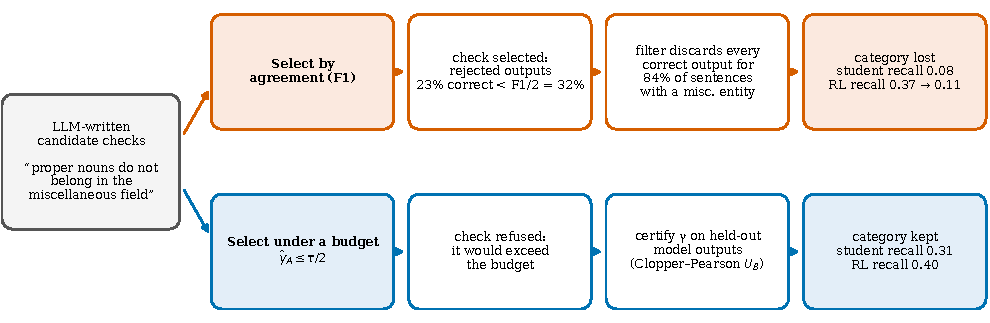
\includegraphics[width=\textwidth]{gen/fig_overview.pdf}
% TikZ alternative with the same numbers: % TikZ version of the overview figure (gen/fig_overview.pdf is the matplotlib
% version used by default). Numbers come from gen/numbers.tex, so both stay in
% sync with the experiment outputs. Needs \usetikzlibrary{arrows.meta} (loaded
% in main.tex). Not compiled in the authoring environment: check after building.
\definecolor{okred}{HTML}{D55E00}
\definecolor{okblue}{HTML}{0072B2}
\definecolor{okgrey}{HTML}{555555}
\begin{tikzpicture}[
    font=\scriptsize,
    every node/.style={align=center},
    box/.style={draw, rounded corners=2pt, line width=0.6pt, text width=2.55cm,
                minimum height=1.15cm, inner sep=2pt},
    arr/.style={-{Stealth[length=1.6mm]}, line width=0.6pt}]
  % source
  \node[box, draw=okgrey, fill=okgrey!8, text width=2.25cm, minimum height=2.6cm] (src) at (1.25,0)
    {LLM-written\\candidate checks\\[3pt]\emph{``proper nouns do not belong in the miscellaneous field''}};
  % agreement path (top)
  \node[box, draw=okred, fill=okred!12] (a1) at (4.25, 0.95) {\textbf{Select by\\agreement (F1)}};
  \node[box, draw=okred]                (a2) at (7.30, 0.95) {check selected:\\rejected outputs \precIEElse{}\\correct $<$ F1/2 $=$ \thrIE};
  \node[box, draw=okred]                (a3) at (10.35,0.95) {filter discards every correct\\output for \frSubPctFoneIEHasElseType\%{} of sentences\\with a misc.\ entity};
  \node[box, draw=okred, fill=okred!12] (a4) at (13.40,0.95) {category lost\\student recall \dsRecFone\\RL recall \rlRecInit{} $\to$ \rlRecFone};
  % budgeted path (bottom)
  \node[box, draw=okblue, fill=okblue!10] (b1) at (4.25,-0.95) {\textbf{Select under a budget}\\$\hat\gamma_A\le\tau/2$};
  \node[box, draw=okblue]                 (b2) at (7.30,-0.95) {check refused:\\it would exceed\\the budget};
  \node[box, draw=okblue]                 (b3) at (10.35,-0.95) {certify $\gamma$ on held-out\\model outputs\\(Clopper--Pearson $\UB$)};
  \node[box, draw=okblue, fill=okblue!10] (b4) at (13.40,-0.95) {category kept\\student recall \dsRecCert\\RL recall \rlRecCert};
  % arrows
  \draw[arr, okred]  (src.east) ++(0,0.3)  -- (a1.west);
  \draw[arr, okblue] (src.east) ++(0,-0.3) -- (b1.west);
  \foreach \x/\y in {a1/a2, a2/a3, a3/a4} \draw[arr, okred]  (\x.east) -- (\y.west);
  \foreach \x/\y in {b1/b2, b2/b3, b3/b4} \draw[arr, okblue] (\x.east) -- (\y.west);
\end{tikzpicture}

\caption{\textbf{Two ways to select LLM-written checks from the same
candidate pool} (CoNLL-2003). Agreement (top) keeps a check whose rejected
outputs are mostly wrong, although they include every correct answer of one
category; the category then disappears from filtered training data, from
what a distilled student recalls and from what an RL policy produces. A
false-rejection budget (bottom) refuses the check, and the selected verifier
is certified on held-out model outputs. RL recall is the mean over four
seeds (\S\ref{sec:downstream}).}
\label{fig:overview}
\end{figure*}

Structured outputs come with cheap checks. A SQL query should execute, an
extraction should validate against its schema, a function call should name
an existing function with well-typed arguments. Conjunctions of such checks
act as \emph{verifiers}: they gate best-of-$N$ selection
\citep{snell2024scaling,brown2024monkeys,stroebl2024verifier}, filter
synthetic training data, and gate rewards in reinforcement learning with
verifiable rewards (RLVR) \citep{shao2024deepseekmath,tinyv2025}. A verifier
therefore decides what models are trained on, and an error that always
rejects one kind of correct answer can remove that kind of answer from what
models learn without showing up in average accuracy. Increasingly, the
checks are written by a language model and kept if they agree with
correctness labels \citep{autopyverifier2026,shankar2024validators} or if
their false-failure rate on a few labelled outputs is small
\citep{shankar2024spade}; related pipelines rank code by agreement with
generated tests \citep{chen2023codet} or validate generated tests against
reference solutions \citep{hardtests2025}.

These criteria count errors in aggregate. None asks \emph{whose} correct
outputs a verifier rejects, although false rejections are rarely spread
evenly: a check encodes an assumption about what correct outputs look
like, and when the assumption is wrong for one kind of input it rejects
all of them. On CoNLL-2003, an LLM-written check states that proper nouns
do not belong in the ``miscellaneous'' field. The category consists of
proper nouns (\emph{German}, \emph{Euro 96}), but models put so many wrong
entities there that the check raises agreement and is selected
(Figure~\ref{fig:overview}, top).
Hand-written checks show the same concentration: a standard morphology
check that segments must concatenate to the word rejects every
canonical segmentation (Appendix~\ref{app:more}).

\paragraph{Key insight.} By the break-even property of F1
\citep{zhao2013beyond,lipton2014optimal}, adding a check raises F1 exactly
when the outputs it newly rejects are correct less than half as often as
the current F1 (Proposition~\ref{prop:f1}), however many correct outputs of
one kind that includes. Deletion therefore needs only a category on which
models are rarely right and a candidate check that isolates it. This makes
it predictable: of our six tasks only CoNLL has both, and adding isolating
checks to Few-NERD reproduces the failure where the condition predicts.

\paragraph{Approach.} We select checks that catch the most wrong outputs
subject to a budget on $\gamma$, the fraction of inputs on which the
verifier rejects some correct output, overall and per group of inputs
(the budget is $\tau$), and certify $\gamma$ on a held-out split of \emph{model} outputs with an exact
binomial bound. Two differences from existing criteria matter. Measuring
false rejection per input gives a quantity that rules out deleting any
category holding more than $2\tau$ of the inputs, named or not, and bounds
what filtering and gated best-of-$N$ can lose
(Proposition~\ref{prop:coverage}). A per-output budget as in SPADE also
prevented deletion in our experiments, but it protects a category only in
proportion to its share of correct outputs, which is small for
categories that models rarely get right.
Certifying on model outputs rather than gold matters because checks can
fail on correct answers that differ from the reference: certified on gold
alone, a SQL verifier claims \ablGoldClaimSQL\% but rejects some correct
output on \rtGoldOnlyTestGammaSQL\% of test inputs (\S\ref{sec:validity}). The statistics themselves are
standard split-sample risk control \citep{angelopoulos2021ltt}.

\paragraph{Contributions.}
(1)~\emph{Diagnosis.} We document category deletion by agreement-selected
verifiers in one natural case and explain it with the break-even property
of F1. On CoNLL, F1
and the AutoPyVerifier objective delete the miscellaneous category whenever
the isolating check is among the candidates, and F1 deletes in at most
\delRateFoneMaxOther\% of selections on the five tasks where the condition
fails. In a Few-NERD stress test F1 takes the \injNPicked\ least precise of
\injNFewnerd\ injected checks, and with a casing check written in a natural
proposer round it removes on average \eOtherFone\% of a Few-NERD category
(\S\ref{sec:deletion}).
(2)~\emph{Consequence.} The deletion is learned. Students distilled from
F1-filtered data recall \dsRecFone\ of the category against \dsRecCert, and
removing only the deleting check restores \ablDelRec; a policy trained with
reinforcement learning and gated by the F1-selected verifier unlearns the
category in all \rlNFone\ seeds, while the certified verifier keeps it
(\S\ref{sec:downstream}).
(3)~\emph{Remedy.} Budgeted selection with a held-out certificate on model
outputs deletes no category on any task or budget, its bound covers the
mean test rate on all six tasks but not SQL under database shift, and its
average accuracy is at most about 3 points below agreement-based selection
(\S\ref{sec:cost}, \S\ref{sec:validity}). Simpler safeguards, a
per-output budget or gold-based admission, also prevented deletion here;
what the certificate adds is a checked bound on model outputs.

% =====================================================================
\section{Related Work}\label{sec:related}
\paragraph{Selecting LLM-written checks.} LLMs write reward code
\citep{ma2024eureka}, unit tests that rerank code \citep{chen2023codet},
labeling functions for weak supervision \citep{scriptoriumws2025}, in the
tradition of data programming \citep{ratner2016data,ratner2017snorkel},
and assertions and verifiers for LLM outputs. How the generated checks are
kept differs. AutoPyVerifier searches for a compact conjunction that
maximises agreement (F1) with correctness labels \citep{autopyverifier2026},
our closest baseline; EvalGen keeps the implementation of each criterion
with the best F1-like alignment to a user's grades
\citep{shankar2024validators}. SPADE selects the smallest set of
LLM-written assertions whose coverage of bad outputs is at least $\alpha$
and whose false-failure rate is below a threshold on a small labelled sample
\citep{shankar2024spade}; our budgeted selection is of the same
constrained form. HardTests validates generated tests against human oracle
programs \citep{hardtests2025}, and CodeContests+ measures how often
generated tests reject correct submissions on real labelled submissions,
noting that checker errors concentrate on problems with several correct
answers \citep{wang-etal-2025-codecontests}. None of these shows that the
selection criterion itself removes a whole category of correct outputs,
follows the effect into training, or gives a held-out bound on false
rejection; we address all three.

\paragraph{Verifier error in RL and filtering.} Rule-based verifiers
produce false negatives and model-based ones can be gamed
\citep{tinyv2025,pitfalls2025verifiers}; false-negative rates of
exact-match verifiers differ across languages \citep{zhou2026multilingual},
and \citet{ray2026fuzzing} fuzzes RLVR verifiers. Random false negatives
mostly slow learning \citep{rad2026rate}. \citet{egashira2026delay} inject
systematic false negatives triggered by a formatting token or by answering
in English and find that the policy first unlearns the triggering behaviour
and then recovers. We study the case where the triggering behaviour is a
correct output category: unlearning it is then a lasting loss, invisible in
average accuracy. Data filters can likewise remove some kinds of text
\citep{gururangan-etal-2022-whose}, and average metrics hide such subgroup
failures \citep{oakdenrayner2020hidden,sagawa2020dro}.

\paragraph{Risk control.} Our selection maximises catch subject to a bound
on false rejection over a finite pool of checks, a Neyman--Pearson-style
problem \citep{rigollet2011neyman}; our certificate is a one-sided
Clopper--Pearson bound \citep{clopper1934,hanley1983rule} on a held-out
split, a standard instance of split-sample risk control
\citep{angelopoulos2021ltt,angelopoulos2024crc}. Conformal methods give
finite-sample guarantees for LM outputs
\citep{quach2024conformal,mohri2024conformal}, including group-conditional
filtering of claims \citep{cherian2024conformal}; SAFER bounds the chance
that correct answers are wrongly excluded when filtering sampled answers
\citep{wang2026safer}, and \citet{kiyani2026cheap} control errors when
routing between cheap and expensive verification. What we certify differs:
the input-level rate at which a verifier built from LLM-written checks
rejects some correct model output, overall and per group.

% =====================================================================
\section{Setup}\label{sec:setup}
An input $x$ has a gold output; a model produces a greedy output $y_0$ and
samples $y_1,\dots,y_N$. A correctness label $C(y)$ decides whether $y$ is
right; a \emph{check} $c(y,x)$ accepts or rejects $y$ without seeing gold;
a \emph{verifier} $V$ is a conjunction of checks. The label must not
presuppose the checks being audited (for SQL, execution match entails ``the
query executes'', so we label by result equivalence on several databases).

Checks are selected on a labelled split A and certified on a disjoint
labelled split B of the same task. Each input $x$ comes with a set $S_x$ of
outputs; on A and B, $S_x$ holds the gold output and, for each generating
model, a greedy output and three samples. Inputs also fall into
\emph{groups}, such as the sentences that contain a given entity type
(\S\ref{sec:method}). Let $Z_x=1$ if $V$ rejects at least one correct
output in $S_x$ (gold counts as correct), and let $R_x$ be the fraction of
the correct outputs in $S_x$ that $V$ rejects. The quantity we control is
$\gamma=\Pr_x[Z_x=1]$ for output sets structured like B's. It is defined
per input because inputs, not outputs, are independent, and because losing
an input entirely is the harm we want to bound. $\gamma_g$ is the same
restricted to a group $g$ of inputs, and $\hat\gamma_A$, $\hat\gamma_B$ are
the empirical fractions on A and B. We also report the
\emph{instance-averaged false-rejection rate} $\bar\delta$, the mean of
$R_x$ over inputs with a correct output in $S_x$, on any output set, and
the \emph{catch rate}, the fraction of incorrect outputs rejected.
\emph{Reject-gated best-of-$N$} returns $y_0$ if $V$ accepts it, else a
uniformly random accepted sample, else $y_0$; we report its expected
accuracy, computed in closed form over that random choice. A \emph{data filter} keeps
the outputs $V$ accepts. An input is \emph{lost} if $V$ rejects every
correct output in $S_x$ (gold included) or, for a training-data filter,
every correct model output; inputs without a correct model output are not
counted. A group is \emph{deleted} when at least half of its inputs are
lost.

% =====================================================================
\section{Why Agreement Deletes Categories}\label{sec:why}
A check trades the correct
outputs it rejects, which lower agreement, against the wrong outputs it
rejects, which raise it. F1 makes the exchange rate explicit: rejecting a
set of outputs pays off whenever that set is less precise than half the
current F1, regardless of whose outputs they are. Formally, let a verifier
$V$ have $\mathrm{F1}(V)=2\,TP/(2\,TP+FP+FN)$ over outputs, gold
included. The following is the set-level form of a known property of F1,
whose break-even precision is $\mathrm{F1}/2$
\citep[Lemma~12]{zhao2013beyond}; it is why the F1-optimal threshold of a
calibrated classifier is half the optimal F1 \citep{lipton2014optimal}.

\begin{figure}[t]\centering
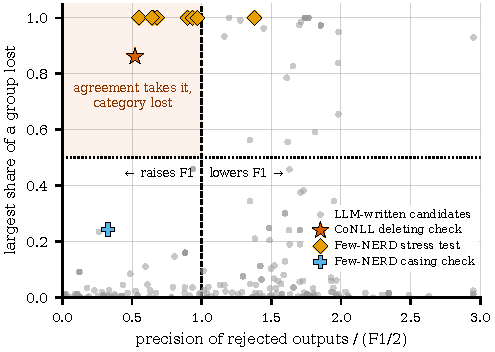
\includegraphics[width=\columnwidth]{gen/fig_mechanism.pdf}
\caption{\textbf{The two ingredients of deletion.} Each point is a candidate
check added alone to the empty verifier on split A (\figMechN\ checks over six
tasks, including the Few-NERD stress-test and feedback-round checks).
$x$: precision of the outputs it rejects relative to the task's break-even
precision F1/2; left of the dashed line the check raises F1
(Proposition~\ref{prop:f1}). $y$: the largest share of a group's inputs it
loses entirely. Only \figMechDanger\ checks fall in the shaded region, where
agreement takes a check that deletes a group: the CoNLL deleting check and
\figMechDangerInj\ injected stress-test checks. \figMechClip\ checks with
$x>3$ are drawn at the right edge.}
\label{fig:mechanism}
\end{figure}

\begin{proposition}\label{prop:f1}
Let a check $c$ newly reject a nonempty set $R$ of outputs that $V$
accepts, a fraction $p$ of which is correct. Then
$\mathrm{F1}(V\wedge c)>\mathrm{F1}(V)$ if and only if
$p<\mathrm{F1}(V)/2$.
\end{proposition}

\noindent In particular, a check that rejects every correct output in a
group raises F1 whenever its rejected outputs fall below this threshold,
however large the group. Since $\mathrm{F1}/2\le1/2$, only checks whose
rejected outputs are mostly wrong qualify, and the threshold rises as F1
selection proceeds. Deletion thus needs two ingredients, a group on which
models are rarely right and a candidate that isolates it
(Figure~\ref{fig:mechanism}), and agreement offers no protection against it. The same algebra gives a break-even
precision of $F_\beta/(1+\beta^2)$ for $F_\beta$, so recall-weighted
agreement ($\beta>1$) is less permissive and accuracy (break-even $1/2$) more
permissive, but no agreement measure asks which outputs are rejected. The
remedy in the next section therefore constrains false rejection directly.
The proposition itself needs no empirical test; \S\ref{sec:deletion} tests
whether the two ingredients occur and whether selection on finite samples
behaves as it implies.


% =====================================================================
\section{Constrained, Certified Selection}\label{sec:method}
The pipeline has three stages: an LLM proposes candidate checks, a subset
is selected on split A under a false-rejection budget, and the selected
verifier is certified on split B.

\paragraph{Propose.} An LLM receives the task definition, how the label
parses outputs, helper functions, training examples with gold and, in later
rounds, correct and incorrect model outputs and split-A feedback; it returns
candidate checks as Python functions. Checks run in a sandbox that hides
gold, restricts imports, limits time and memory, and fails closed.

\paragraph{Select (split A).} Starting from the empty conjunction, greedily
add the check (LLM-written or hand-written) that catches the most additional
incorrect outputs on A, subject to $\hat\gamma_A\le\tau/2$ and, in the
\emph{group} variant, $\hat\gamma_{g,A}\le\tau/2$ for every group with at
least 50 inputs; ties are broken by candidate order, and selection stops when
no admissible check catches anything more. The empirical budget is $\tau/2$
rather than $\tau$ so that the upper bound on B, which exceeds the
empirical rate, can still fall below $\tau$. Groups are fixed before
selection: subgroups defined from gold (for example the entity types
present) and eight clusters of character $n$-gram TF-IDF vectors of the
inputs, which need no gold. The overall constraint already protects every
large enough group, named or not (Proposition~\ref{prop:coverage}(c)), so
our main verifier uses it alone; the group variant, which adds protection
for smaller named groups, is evaluated alongside it
(Table~\ref{tab:safety}).

\paragraph{Certify (split B).} On a disjoint split B of $n=1{,}000$
inputs, let $k$ be the number of inputs on which $V$ rejects a correct
output. The certificate is the one-sided Clopper--Pearson upper bound $\UB$
on $\gamma$ at level $1-0.05/3$, Bonferroni-corrected over the three
budgets $\tau\in\{1,2,5\}\%$ because the reported budget is chosen on B:
per task, the smallest $\tau$ with $\UB\le\tau$, a rule fixed in advance
(if none qualified, no verifier would be certified; this did not occur).
The group certificate additionally requires the bound of every group with
at least 50 inputs on B, at level $1-0.05/(3G)$ for $G$ such groups, to be
at most 20\%; budgets of 1--5\% cannot be certified per group at this size,
so this level was set from the bound arithmetic, not from results
(Appendix~\ref{app:validity}).

\paragraph{Validity.} Because the three candidate verifiers depend only
on split A and proposal data, and B's inputs are drawn i.i.d.\ and
independently of A, $k\sim\mathrm{Bin}(n,\gamma)$ for each of them, so each
bound covers its $\gamma$ with probability $1-0.05/3$ and, by a union bound,
all three hold together with probability at least $0.95$
\citep{clopper1934}. The guarantee is about B's distribution of inputs and
model outputs.

\paragraph{What $\gamma$ controls.} We budget $\gamma$ because every harm
of a false rejection that we care about requires some input to have a
correct output rejected; $\gamma$ is the probability of that event, so it
bounds each harm at once.

\begin{proposition}\label{prop:coverage}
For inputs and output sets drawn like B's:
(a)~a data filter applied to the model outputs in $S_x$ loses, in
expectation, at most a fraction $\gamma$ of inputs, and $\bar\delta\le\gamma$;
(b)~for each of the three models, reject-gated best-of-$N$ has accuracy at
least $p_0-\gamma$ for every $N$, where $p_0$ is the accuracy of the
model's greedy output $y_0$;
(c)~if at least half of the inputs of a group holding a fraction $s$ of
all inputs are lost, then $\gamma\ge s/2$ and $\gamma_g\ge 1/2$; the same
holds for the empirical $\hat\gamma$ on any finite set of inputs.
\end{proposition}

\noindent Part (c) links the budget to deletion: a verifier with
$\gamma\le\tau$ cannot delete any group holding more than $2\tau$ of the
inputs, named or not, and the group certificate ($\gamma_g\le20\%$) rules
out deleting any certified group. The protection is limited: at
$\tau=5\%$ only groups holding more than 10\% of inputs are guaranteed.
At the resampling budget of $\tau=2\%$, selection on A cannot delete any
group holding more than 2\%, and since our groups hold at least 5\% of
inputs this predicts that budgeted selection deletes none of them, which
\S\ref{sec:cost} tests (details in Appendix~\ref{app:validity}). Part (a) applies to
B-like output sets; the $\bar\delta$ we report on test pools with 33
outputs per model is related to $\gamma$ but not formally bounded by it.

\noindent Proofs are in Appendix~\ref{app:proofs}. The certificate is
distributional: it holds for the distribution B is drawn from, and transfer
to other test sets and models is an empirical question (\S\ref{sec:validity}).

% =====================================================================
\section{Experimental Setup}\label{sec:exp}
\paragraph{Tasks.} Six structured tasks with exact labels: entity
extraction on CoNLL-2003 \citep{tjongkimsang2003conll} and Few-NERD
\citep{ding2021fewnerd} (JSON with four and eight entity fields); function
calling on Glaive v2 \citep{glaive2023fc} (exact name and type-strict
argument match); text-to-SQL on Spider \citep{yu2018spider} (result
equivalence on the original and three perturbed databases); GSM8K
\citep{cobbe2021gsm8k} (final answer); and SIGMORPHON 2022 English
segmentation \citep{batsuren2022sigmorphon}.

\paragraph{Models and data.} GPT-4o-mini, Llama-3.1-70B and Qwen2.5-72B.
Splits A and B hold 1{,}000 disjoint training inputs each, with gold plus a
greedy output and three samples (temperature 0.7) per model. For CoNLL, SQL,
GSM8K and morphology, three test draws of 200 inputs were used during
development; accuracy results are on a \emph{fresh} draw of 300 inputs
never inspected before the selections were frozen (greedy plus 32 samples
per model), while the validity check (\S\ref{sec:validity}) and the
ablations use the development draws. For Few-NERD and function calling, which were added
later, the three test draws of 200 inputs were generated after the
selections were frozen and never inspected during development; they are
pooled (600 inputs) as the final test set.
Weaker generators (Llama-3.1-8B, Qwen2.5-7B) provide fresh outputs for SQL
and GSM8K to test transfer to models absent from A and B.

\paragraph{Candidates.} GPT-4o and Claude Opus~5.5 propose \candTotal\
checks in total. For GSM8K one proposer round was guided toward checks of
the stated arithmetic, and the SQL and morphology task descriptions encode
lessons from split-A feedback; all prompts are released with the code.

\paragraph{Baselines.} \emph{Hand-written}: standard well-formedness stacks
(Appendix~\ref{app:impl}). \emph{F1-selected}: greedy selection
maximising the F1 of ``accepted'' as a predictor of ``correct''.
\emph{F1 with budget}: the same under our input-level budget.
\emph{Per-output budget}: maximum catch subject to a false-failure rate
over correct model outputs at most $\tau/2$ on A, the constraint of SPADE
\citep{shankar2024spade}.
\emph{AutoPyVerifier objective} (APV): the selection rule of
\citet{autopyverifier2026} taken from the authors' code (macro-F1,
feasibility via Hoeffding bounds on both predictive values, smallest
feasible bundle), applied greedily to our candidate pool; their LLM
critique-and-refine search is not reproduced.

% =====================================================================
\section{Results}\label{sec:results}
\subsection{Diagnosis: agreement deletes categories where predicted}\label{sec:deletion}

\begin{table*}[t]\centering\footnotesize
\setlength{\tabcolsep}{3.4pt}
\begin{tabular}{@{}l cccc c cccc c cccc@{}}
\toprule
& \multicolumn{4}{c}{Catch rate on B (\%)} & & \multicolumn{4}{c}{B inputs with a correct output rejected (of 1000)} & & \multicolumn{4}{c}{Group deleted in resampling (\% of 200)} \\
\cmidrule(lr){2-5}\cmidrule(lr){7-10}\cmidrule(lr){12-15}
Task & Hand & F1 & APV & Cert. & & Hand & F1 & APV & Cert. & & F1 & APV & Budget & Group \\
\midrule
CoNLL & 13.4 & 64.0 & 64.1 & 52.5 &  & 3 & 178 & 179 & 26 &  & 69 & 69 & 0 & 0 \\
Few-NERD & 14.5 & 27.0 & 0.0 & 28.2 &  & 3 & 7 & 0 & 29 &  & 0 & 0 & 0 & 0 \\
Func.\ call & 70.2 & 76.8 & 76.8 & 71.7 &  & 4 & 12 & 12 & 8 &  & 0 & 0 & 0 & 0 \\
SQL & 13.6 & 23.0 & 38.3 & 20.4 &  & 2 & 25 & 152 & 10 &  & 0 & 3 & 0 & 0 \\
GSM8K & 35.2 & 9.5 & 11.3 & 9.7 &  & 455 & 1 & 15 & 1 &  & 0 & 0 & 0 & 0 \\
Morph. & 24.3 & 2.8 & 0.0 & 2.8 &  & 282 & 1 & 0 & 8 &  & 0.5 & 0 & 0 & 0 \\

\bottomrule
\end{tabular}
\caption{\textbf{Catch, false rejection and category deletion.} APV: the
AutoPyVerifier selection objective. Cert.: budgeted selection at each
task's smallest certified budget (5\% for CoNLL and Few-NERD, 1\% for
GSM8K, 2\% otherwise). Resampling: 200 bootstrap replicates of split A,
each with a random 70\% of the LLM-written candidates plus all hand-written
ones; Budget (input-level budget) and Group (per-group variant) select at
$\tau=2\%$; a group (at least 50 inputs on
B) is deleted when at least half of its inputs lose every correct output
on B.}
\label{tab:safety}
\end{table*}

We first test whether agreement-based selection deletes categories, and
where (Table~\ref{tab:safety}). On CoNLL, it deletes a group in \delRateFoneIE\% of resampled selections with F1 and \delRateApvIE\% with the
AutoPyVerifier objective. The deleted group is the miscellaneous category:
on the fresh draw, the F1-selected verifier as a data filter removes every
correct output for \frSubFoneIEHasElseType\ such inputs, the certified one
for \frSubCertIEHasElseType. The rate is set by the resampling protocol:
the deleting check survives the 70\% candidate subsample in \rdAvailIE\ of
\rdNIE\ replicates, and both objectives delete the category in
\rdDelAvailFoneIE\% of those replicates and in \rdDelNotFoneIE\% of the
others.

\paragraph{Alternative explanations.} The rejected outputs are not label
errors: the check rejects the gold answer itself for \advGoldRejA\% (A)
and \advGoldRejB\% (B) of sentences with a miscellaneous entity. More
labelled data does not help: F1 selection on A and B together still takes
the check, and \advABmin--\advABmax\% of such sentences in the test pools
lose every correct output. Gold-defined groups are not needed to see it:
the input clusters richest in such sentences lose
\advClRichMin--\advClRichMax\% of their inputs, the others at most
\advClPoorMax\%. Nor does the conclusion hinge on the 50\% threshold: the
worst group loses on average \worstMeanFoneIE\% of its inputs under F1
against \worstMeanBudgetIE\% under budgeted selection.

\paragraph{Where deletion occurs.} On the other five tasks the deletion
rate is at most \delRateApvSQL\% (the AutoPyVerifier objective on SQL,
which also rejects a correct output on \gammaKApvSQL\ of 1{,}000 SQL inputs
and selects nothing on morphology and Few-NERD). Proposition~\ref{prop:f1}
explains the pattern. On split A, the outputs for CoNLL inputs with a
miscellaneous entity are correct at rate \precIEElse, below the threshold \thrIE, and one
candidate isolates them; F1 computed without gold outputs selects the same
check. Few-NERD has \nDeletableFewnerd\ groups below its
threshold and morphology \nDeletableMorph, but no candidate isolates them
at low enough precision (F1 deleted in \delRateFoneMaxOther\% of morphology
selections); function calling, SQL and GSM8K have no group
below threshold, so checks that reject a whole group's correct outputs
there lower F1 and are never
selected.

\paragraph{Stress test.} To test the prediction, we added \injNFewnerd\
checks to the Few-NERD pool, one per entity type, each rejecting every
output that lists an entity of that type (written by us, not by the
proposer). The initial threshold on Few-NERD is \thrFewnerd, and it rises
during selection. F1 selection took the \injNPicked\ whose rejected outputs were
correct at rate at most \injPrecPickedMax\ (\injPicked), and none of those
with rate \injPrecUnpickedMin\ or more. It then deleted a group in
\injDelFone\% of resampled selections, losing \injWipedFone\% of the
inputs with a \injWipedGroupFone\ entity on B and rejecting a correct output on
\injGammaKFone\ of 1{,}000 inputs. Budgeted, F1-with-budget and
group-constrained selection took none of the injected checks at any budget
and deleted nothing (\injDelBudget\%). A control on SQL, a check
rejecting every query with a join (rejected outputs correct at rate
\injPrecSQL, above the threshold \thrSQL), was never selected.

\paragraph{A natural feedback round.} To see whether proposers write such
checks unprompted, we ran one more Few-NERD round in which GPT-4o and
Claude Opus received the usual split-A feedback on unsound checks (no
mention of categories) and wrote \eNnew\ new candidates, kept out of all
other results. GPT-4o's \emph{entities\_with\_proper\_casing} rejects any
all-lowercase entity because ``proper nouns usually begin with capital
letters''; Few-NERD's \emph{other} type contains many lowercase entities
(diseases, chemicals). Across 200 resampled selections, F1 selection
removed on average \eOtherFone\% of the inputs with an \emph{other}
entity (90th percentile \eOtherPnineFone\%), short of deletion,
against \eOtherBudget\% for budgeted selection, \eOtherGroup\% for the
group variant and \eOtherOutlvl\% for a per-output budget. The
AutoPyVerifier objective deleted a group in \eDelApv\% of selections by
taking two faulty checks that reject almost every output:
with most outputs wrong, its macro-F1 rewards rejecting nearly everything.
F1 refused both, as Proposition~\ref{prop:f1} predicts.

\subsection{Consequence: deleted categories are learned}\label{sec:downstream}

\begin{figure}[t]\centering
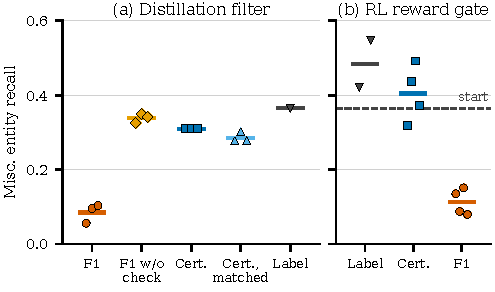
\includegraphics[width=\columnwidth]{gen/fig_downstream.pdf}
\caption{\textbf{The deleted category is learned} (CoNLL test, \szEvalIE\ inputs;
one point per training seed or subsample, bar at the mean).
(a)~Qwen3-0.6B students distilled from the outputs each filter keeps. F1:
the F1-selected verifier; F1~w/o check: the same without its deleting
check; Cert.: the certified verifier (its three seeds give identical
recall); Cert., matched: the certified set subsampled to the F1 set's size;
Label: correct outputs only. (b)~Policies trained with GRPO for 200 steps
from the label-filtered student, with the reward gated by each verifier or
by the label alone; the dashed line is the starting recall. Overall
accuracy is similar across conditions (distillation \dsAccFone\% vs
\dsAccCert\% for F1 vs certified; RL \rlAccFone\% vs \rlAccCert\%); full
results in Appendix Table~\ref{tab:down}.}
\label{fig:down}
\end{figure}

\emph{Distillation} (Figure~\ref{fig:down}a). A student trained on
F1-filtered data reaches similar overall accuracy to one trained on
certified-filtered data but recalls \dsRecFone\ of miscellaneous entities
against \dsRecCert\ (three seeds). The F1-filtered data still contains
\advMiscNFone\ miscellaneous entities, but none is title-case and
\advMiscPrecFone\% are correct, against \advMiscTitleCert\% title-case and
\advMiscPrecCert\% correct with certified filtering. The student follows
the data: on the test set it predicts \stuMiscNFone\ miscellaneous entities
(certified: \stuMiscNCert), of which \stuMiscTitleFone\% are title-case
(certified: \stuMiscTitleCert\%). The quantity alone is not the
cause: the label-filtered set has fewer (\advMiscNOracle, all correct) and
its student recalls \rlRecInit. The cause is the deleting check itself: removing only
that check from the F1 filter restores recall to \ablDelRec\
(\ablDelRecMin--\ablDelRecMax\ over \ablDelN\ seeds) at similar accuracy
(\ablDelAcc\%).

The gap is not a data-size effect: subsampling the certified set to
the F1 set's size keeps a recall of \dsMatchedRec\ (three subsamples), and
a 1.7B student shows the same pattern (\dsBigRecCert\ vs \dsBigRecFone\
recall at \dsBigAccCert\% vs \dsBigAccFone\% accuracy). On Few-NERD, where no selector deletes a
category, certified filtering is level with F1 filtering
(\fnSeedCert$\pm$\fnSeedSdCert\ vs \fnSeedFone$\pm$\fnSeedSdFone\ over
\fnSeedN\ seeds) and above hand-written filtering (\fnAccHw, one seed;
paired difference \fnDiffHw\ for the first seed).

\emph{Reinforcement learning} (Figure~\ref{fig:down}b). We train policies
with GRPO \citep{shao2024deepseekmath} from a student that already
recognises miscellaneous entities (recall
\rlRecInit). With the label as reward, RL keeps or improves the category
(\rlRecLabel), and gating the reward with the certified verifier keeps it
near its starting level (\rlRecCert; \rlRecMinCert--\rlRecMaxCert\
across \rlNCert\ seeds). Gating it with the F1-selected verifier makes the
policy unlearn the category in every seed (\rlRecFone, at most
\rlRecMaxFone). Because the reward requires the verifier's acceptance,
this is the expected mechanism; the experiment measures its size and
whether average accuracy reveals it. It does not: F1-gated policies end at
\rlAccFone\% accuracy against \rlAccInit\% at the start, while
certified-gated ones reach \rlAccCert\%. \citet{egashira2026delay} found that a policy
unlearns the behaviour that triggers systematic false negatives and then
recovers; here that behaviour is producing a correct category, so the
unlearning is itself the loss, and average accuracy does not show it.
Starting from the base model, every reward, including
the label alone, removed the category, because the base model rarely
produced correct miscellaneous entities (recall \rlRecBase;
Appendix~\ref{app:rl}).

\subsection{Remedy: no deletion, little cost}\label{sec:cost}
\paragraph{Deletion.} As Proposition~\ref{prop:coverage}(c) predicts,
budgeted, group-constrained and F1-with-budget selection deleted in none of
\nRepTotal\ resampled selections (Table~\ref{tab:safety}), so the protection
comes from the constraint, not the objective. Resampling rates describe
how stable selection is; the replicates share split B and are not
independent samples, so we attach no confidence intervals to them. A per-output budget never deletes either (\rdDelOutlvlMax\% on
all six tasks and in the stress test),
with similar catch (\rdCatchOutlvlIE\% vs \rdCatchBudgetIE\% on CoNLL). The
result does not depend on the budget: at $\tau=1\%$ and $5\%$ (the budget
of the certified CoNLL and Few-NERD verifiers), no budgeted variant deleted
a group on any task, and under budgeted selection the worst group lost
at most \bsWorstMax\% of its inputs. A simpler safeguard also works on our
data: admitting only checks that reject no gold answer on A, then
selecting by F1, never takes the CoNLL casing check (it rejects the gold
answer for \advGoldRejA\% of sentences with a miscellaneous entity) and
deletes no group on any task. It gives no guarantee, however: checks that
fail only on correct answers that differ from gold pass this test, which is
how gold-only certification fails on SQL (\S\ref{sec:validity}). Finally,
a budget is spent, not saved: on Few-NERD and morphology the certified
verifier rejects a correct output on more B inputs than F1 does
(Table~\ref{tab:safety}), in exchange for catch.

\begin{table*}[t]\centering\footnotesize
\setlength{\tabcolsep}{3.6pt}
\begin{tabular}{@{}llccccccccc@{}}
\toprule
& & \multicolumn{5}{c}{Gated best-of-32 accuracy (\%)} & & \multicolumn{3}{c}{Test $\bar\delta$ (\%)} \\
\cmidrule(lr){3-7}\cmidrule(lr){9-11}
Task & Model & Base & Hand & F1 & APV & Cert. & Cert.\ $-$ F1 & F1 & APV & Cert. \\
\midrule
\multirow{3}{*}{CoNLL} & Llama-3.1-70B & 38.7 & 45.5 & 54.2 & 54.2 & 51.8 & $-$2.5 [$-$5.6, +0.5] & 11.9 & 11.9 & 2.0 \\
 & GPT-4o-mini & 36.3 & 36.3 & 42.0 & 42.0 & 41.7 & $-$0.3 [$-$2.0, +1.4] & 7.3 & 7.3 & 0.7 \\
 & Qwen2.5-72B & 49.2 & 49.5 & 52.4 & 52.4 & 53.1 & +0.6 [$-$0.1, +1.7] & 5.1 & 5.1 & 1.1 \\
\addlinespace[2pt]
\multirow{3}{*}{Few-NERD} & Llama-3.1-70B & 34.0 & 34.7 & 36.4 & 34.0 & 36.3 & $-$0.2 [$-$0.5, +0.0] & 0.5 & 0.0 & 2.5 \\
 & GPT-4o-mini & 24.0 & 24.8 & 25.7 & 24.0 & 25.7 & +0.0 [+0.0, +0.0] & 0.0 & 0.0 & 1.8 \\
 & Qwen2.5-72B & 32.8 & 33.9 & 34.6 & 32.8 & 34.6 & +0.0 [$-$0.5, +0.5] & 0.0 & 0.0 & 1.1 \\
\addlinespace[2pt]
\multirow{3}{*}{Func.\ call} & Llama-3.1-70B & 39.5 & 42.2 & 42.0 & 42.0 & 41.7 & $-$0.3 [$-$0.8, +0.0] & 0.4 & 0.4 & 1.2 \\
 & GPT-4o-mini & 92.5 & 92.5 & 92.8 & 92.8 & 92.8 & +0.0 [+0.0, +0.0] & 0.0 & 0.0 & 0.4 \\
 & Qwen2.5-72B & 95.3 & 95.3 & 95.5 & 95.5 & 95.3 & $-$0.2 [$-$0.5, +0.0] & 0.2 & 0.2 & 0.5 \\
\addlinespace[2pt]
\multirow{3}{*}{SQL} & Llama-3.1-70B & 69.3 & 74.0 & 74.6 & 74.8 & 74.3 & $-$0.3 [$-$1.0, +0.0] & 1.4 & 8.2 & 0.6 \\
 & GPT-4o-mini & 75.0 & 76.0 & 76.0 & 76.7 & 76.0 & +0.0 [+0.0, +0.0] & 1.6 & 9.7 & 1.2 \\
 & Qwen2.5-72B & 76.7 & 77.4 & 77.7 & 78.1 & 77.4 & $-$0.3 [$-$1.0, +0.0] & 1.0 & 9.1 & 0.6 \\
\addlinespace[2pt]
\multirow{3}{*}{GSM8K} & Llama-3.1-70B & 95.3 & 95.3 & 95.6 & 95.6 & 95.6 & +0.0 [+0.0, +0.0] & 0.0 & 0.5 & 0.3 \\
 & GPT-4o-mini & 92.3 & 93.2 & 93.0 & 93.0 & 93.0 & +0.0 [+0.0, +0.0] & 0.0 & 0.3 & 0.3 \\
 & Qwen2.5-72B & 93.3 & 94.4 & 94.5 & 94.5 & 94.5 & +0.0 [+0.0, +0.0] & 0.0 & 0.4 & 0.3 \\
\addlinespace[2pt]
\multirow{3}{*}{Morph.} & Llama-3.1-70B & 34.7 & 33.0 & 34.8 & 34.7 & 34.8 & +0.0 [+0.0, +0.0] & 0.0 & 0.0 & 0.0 \\
 & GPT-4o-mini & 39.7 & 38.4 & 39.7 & 39.7 & 39.7 & +0.0 [+0.0, +0.0] & 0.0 & 0.0 & 0.0 \\
 & Qwen2.5-72B & 39.7 & 38.7 & 39.8 & 39.7 & 39.8 & +0.0 [+0.0, +0.0] & 0.0 & 0.0 & 0.0 \\

\bottomrule
\end{tabular}
\caption{\textbf{Fresh, untouched test data} (300 inputs; 600 for Few-NERD
and function calling; selections frozen beforehand). Brackets: 95\% paired
bootstrap intervals over inputs. Test $\bar\delta$: instance-averaged
false-rejection rate over all 33 outputs per model, related to but not
formally bounded by $\gamma$ (Proposition~\ref{prop:coverage}); for
reference, the certified bounds on $\gamma$ are \boundBIE\% (CoNLL), \boundBFewnerd\% (Few-NERD), \boundBFC\% (function
calling), \boundBSQL\% (SQL), \boundBMath\% (GSM8K), \boundBMorph\%
(morphology).}
\label{tab:fresh}
\end{table*}

\paragraph{Accuracy.} The constraint costs little average accuracy
relative to agreement-based selection (Table~\ref{tab:fresh};
Appendix Figure~\ref{fig:cost}). On CoNLL, where agreement deletes a
category, the certified verifier trails F1 selection for Llama by
\frVsFoneIELlama\ points on the fresh draw ([\frVsFoneLoIELlama,
\frVsFoneHiIELlama]) and \devVsFoneIELlama\ on the three development draws
([\devVsFoneLoIELlama, \devVsFoneHiIELlama]), the largest cost we
observed. The F1 and
AutoPyVerifier-selected verifiers reach their average while rejecting
\frDltFoneIELlama\% of each input's correct outputs on average, against \frDltCertIELlama\% for ours: the average hides whose
answers are rejected. On the other five tasks the certified and F1-selected
verifiers tie. Against hand-written checks, the certified verifier gains
\frGainIELlama, \frGainIEMini\ and \frGainIEQwen\ points on CoNLL and
\frGainFewnerdLlama, \frGainFewnerdMini\ and \frGainFewnerdQwen\ on Few-NERD
(the last interval touches zero); synthesised checks add little elsewhere
(Appendix~\ref{app:more}). We do not claim an average-accuracy advantage
over agreement-based selection.

\subsection{Remedy: does the certificate hold?}\label{sec:validity}
On test pools restructured like split B, the mean over the three test
draws stayed below the certified bound on all six tasks
(Appendix Table~\ref{tab:validity} and Figure~\ref{fig:validity}). Single 200-input draws, whose sampling
error is of the order of the bounds, exceeded it on Few-NERD, SQL and
GSM8K (largest: \valMaxCertFewnerd\% against \valUCertFewnerd\% on
Few-NERD). On the fresh draws, which were never inspected, restructured
the same way, the certified verifier's $\gamma$ stayed below its bound on
CoNLL (\rtFreshIE\%), GSM8K (\rtFreshMath\%) and morphology
(\rtFreshMorph\%) but exceeded it on SQL (\rtFreshSQL\% against
\boundBSQL\%). Across resampled selections the test value fell below
$\UB$ in at least \covCertMath\% of replicates on five tasks but only
\covCertSQL\% on SQL: Spider's test questions use databases unseen in
training, and the guarantee does not fully transfer across that shift.
Bounds of non-certified verifiers can fail outright: the hand-written
GSM8K stack's mean test value is \valMeanHwMath\% against a bound of
\valUHwMath\%. The group certificate passed on \rtGroupCertN\ of six tasks;
on CoNLL the worst group's bound was \rtGroupUIE\%, just above 20\%. On SQL outputs of
weaker models never in A or B, for which the certificate makes no formal
claim, the certified verifier rejected \wkDltCertSQLLlamaeight\% and
\wkDltCertSQLQwenseven\% of their correct outputs per input, below its
bound of \wkBoundSQL\%.

Certifying on model outputs rather than gold is what makes the bound
meaningful. Validating checks against gold answers alone, the
HardTests-style alternative, certifies \ablGoldClaimSQL\% on SQL, yet the
resulting verifier rejects some correct output on \rtGoldOnlyTestGammaSQL\%
of inputs in the like-with-like test pools (\rtGoldOnlyRatioSQL-fold): an
admitted check requires table aliases in joins, which \sqlJoinAlias\ of the
\sqlJoinN\ gold queries with joins in our splits use and many correct model
queries do not
(Appendix~\ref{app:ablate}).

% =====================================================================
\section{Conclusion}
Selecting LLM-written checks by agreement with labels can delete a category
of correct outputs while improving the average, and students and RL
policies then lose the category too. We observed this naturally on one of
six tasks; how often it arises elsewhere remains open, but when it arises
is predictable: agreement rewards any check whose rejected outputs are correct
less than half as often as the current F1. Budgeting false rejection during
selection prevents it at little average cost, and certifying the per-input
rate on held-out model outputs tells a user that the budget held. More
broadly, pipelines that keep generated tests, rubrics or filters by
agreement should report which correct outputs they reject, not only how
many.

\section*{Limitations}
\paragraph{Distributional guarantee.} The certificate covers inputs and
model outputs drawn like split B. It held on held-out test pools of the
same models, but under Spider's train-to-dev database shift coverage over
resamples was \covCertSQL\%, below the nominal 95\%, and the restructured
fresh SQL draw exceeded the bound; a new domain needs its own certification split. For
models absent from B, and for the $\bar\delta$ we report on test pools with
33 outputs per model, it makes no formal claim.
\paragraph{How often deletion occurs.} Proposition~\ref{prop:f1} is exact
for F1; the AutoPyVerifier objective (macro-F1 under feasibility
constraints) deleted the same CoNLL category but is not covered by it.
CoNLL's miscellaneous class is also its least consistently annotated, which
may lower the measured correctness of these outputs, although the deleting
check rejects the gold answers themselves. Natural deletion appeared in one
of six initial candidate pools, and one
extra Few-NERD feedback round produced a check that removed about a third
of a category under F1; the stress-test checks were written by us and show
what selection does with such a candidate, not how often a proposer writes
one. Synthesised checks help mainly on entity extraction.
\paragraph{Scale and data.} Splits of 1{,}000 inputs limit per-group bounds
to about 6--20\%, so the group certificate is coarse and small groups can
be lost within it. All tasks are in English, and the generating models may
have seen these public benchmarks, which affects accuracy levels but not
the comparison between selectors on the same outputs. The development test
draws were inspected, and for four tasks they are also the pools of the
certificate check; accuracy is reported on fresh draws (for Few-NERD and
function calling, on uninspected draws that also serve the certificate
check). One GSM8K proposer round was guided toward arithmetic checks.
\paragraph{Baselines and students.} We reproduce AutoPyVerifier's selection
objective, not its LLM refinement loop, whose critic might have rejected
some of the faulty checks its objective selects; our per-output budget
follows SPADE's constraint but maximises catch instead of minimising the
number of checks. Students are 0.6B and 1.7B models trained with LoRA for
one epoch (the 1.7B result has one seed); RL uses 200 GRPO steps and two to
four seeds.

\section*{Ethical Considerations}
Public benchmarks are used under their licences; no human data is
collected. LLM-written code runs in a restricted sandbox. A certified
verifier is not a correctness guarantee for any single output. AI assistants
were used for coding and drafting; every number is generated from the saved
experiment outputs by a script released with the code.

\bibliography{refs}

\appendix
\section{Proofs}\label{app:proofs}
\paragraph{Proposition~\ref{prop:coverage}.} All statements are about
inputs and output sets drawn like B's, with $\gamma=\mathbb{E}Z_x$.
(a)~An input is lost when every correct model output in $S_x$ is removed;
then $V$ rejects a correct output of $x$, so $\mathbb{1}[x\text{ lost}]\le
Z_x$ pointwise and the expected fraction lost is at most $\gamma$. Also
$R_x\le Z_x$ pointwise, since $R_x>0$ implies $Z_x=1$, so
$\bar\delta\le\gamma$. (b)~Gated selection returns $y_0$ whenever $V$
accepts it, so it is correct whenever $y_0$ is correct and accepted, and
its accuracy is at least $p_0-\Pr[C(y_0)=1,V(y_0)=0]$. Since $y_0\in S_x$,
the event $C(y_0)=1,V(y_0)=0$ implies $Z_x=1$, so the deficit is at most
$\gamma$. (c)~Each lost input has $Z_x=1$; if at least half of group $g$
is lost, $\gamma_g\ge1/2$, and since $g$ holds a fraction $s$ of inputs,
$\gamma\ge s/2$. The argument is the same for empirical frequencies.
\hfill$\square$

\paragraph{Proposition~\ref{prop:f1}} (included for completeness;
cf.\ \citealp{zhao2013beyond}). Let $D=2\,TP+FP+FN$, so
$\mathrm{F1}=2\,TP/D$, and let $R$ contain $t$ correct and $f$ incorrect
outputs, $t+f>0$, $p=t/(t+f)$. Adding $c$ gives $TP'=TP-t$, $FP'=FP-f$,
$FN'=FN+t$ and $D'=D-t-f$. Gold outputs are correct, so $TP+FN\ge1$ and
$TP'+FN'\ge1$, hence $D,D'>0$ and we may cross-multiply:
$2\,TP'/D'>2\,TP/D$ iff
$(TP-t)\,D>TP\,(D-t-f)$ iff $t\,D<TP\,(t+f)$ iff $p<TP/D=\mathrm{F1}/2$.
\hfill$\square$

\section{Certification and Validity Details}\label{app:validity}
\paragraph{Group level.} The group bounds are valid conditionally on the
group sizes, which do not depend on the verifier. With the correction
$0.05/(3G)$, a group of 50 inputs has a bound of about 12\% even with no
errors, and every group we track has one above 6\%, so per-group budgets
of 1--5\% cannot be certified with 1{,}000 inputs.
\begin{figure}[h]\centering
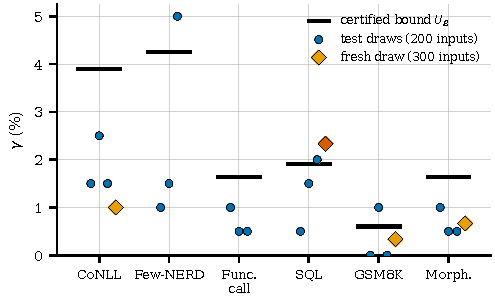
\includegraphics[width=\columnwidth]{gen/fig_validity.pdf}
\caption{Certified bound $\UB$ of the certified verifier (bar) against
$\gamma$ on test pools restructured like split B: the three test draws
(circles) and the fresh draw (diamonds; CoNLL, SQL, GSM8K and morphology).
The fresh SQL draw exceeds its bound (dark diamond), consistent with
Spider's train-to-dev database shift.}
\label{fig:validity}
\end{figure}

\begin{figure}[h]\centering
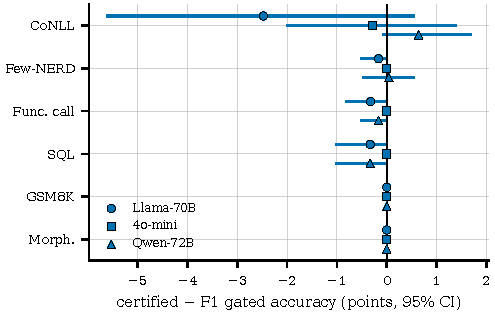
\includegraphics[width=\columnwidth]{gen/fig_cost.pdf}
\caption{Certified minus F1-selected gated best-of-32 accuracy on fresh
test data, with 95\% paired bootstrap intervals, per task and generating
model. The largest cost is on CoNLL for Llama-3.1-70B.}
\label{fig:cost}
\end{figure}

\paragraph{Why budgeted selection does not delete.} In selection,
$\hat\gamma_A\le\tau/2$ rules out deleting on A any group larger than
$\tau$ (Proposition~\ref{prop:coverage}(c)); our groups hold at least 5\%
of inputs, so at the resampling budget of 2\% none can be deleted on A. On
B, the full-data selections at that budget have $\hat\gamma_B\le2\%$, so
deleting a group there would need it to hold under 4\% of inputs, fewer
than the 50 we track.

\begin{table}[h]\centering\footnotesize
\setlength{\tabcolsep}{2.6pt}
\begin{tabular}{@{}llcccc@{}}
\toprule
& & & \multicolumn{2}{c}{Test $\gamma$ (\%)} & \\
\cmidrule(lr){4-5}
Task & Verifier & $\UB$ (\%) & mean & max & Holds \\
\midrule
CoNLL & Hand-written & 0.93 & 0.67 & 1.00 & yes \\
 & F1-selected & 20.53 & 16.50 & 21.50 & yes \\
 & AutoPyVerifier obj. & 20.64 & 16.50 & 21.50 & yes \\
 & Certified & 3.89 & 1.83 & 2.50 & yes \\
\addlinespace[2pt]
Few-NERD & Hand-written & 0.93 & 0.33 & 1.00 & yes \\
 & F1-selected & 1.51 & 0.67 & 1.00 & yes \\
 & AutoPyVerifier obj. & 0.41 & 0.00 & 0.00 & yes \\
 & Certified & 4.25 & 2.50 & 5.00 & yes \\
\addlinespace[2pt]
Func.\ call & Hand-written & 1.08 & 0.00 & 0.00 & yes \\
 & F1-selected & 2.17 & 1.50 & 2.50 & yes \\
 & AutoPyVerifier obj. & 2.17 & 1.50 & 2.50 & yes \\
 & Certified & 1.64 & 0.67 & 1.00 & yes \\
\addlinespace[2pt]
SQL & Hand-written & 0.77 & 0.50 & 1.00 & yes \\
 & F1-selected & 3.77 & 2.17 & 3.00 & yes \\
 & AutoPyVerifier obj. & 17.78 & 14.50 & 15.50 & yes \\
 & Certified & 1.91 & 1.33 & 2.00 & yes \\
\addlinespace[2pt]
GSM8K & Hand-written & 48.91 & 53.00 & 57.50 & \textbf{no} \\
 & F1-selected & 0.60 & 0.00 & 0.00 & yes \\
 & AutoPyVerifier obj. & 2.55 & 1.83 & 2.00 & yes \\
 & Certified & 0.60 & 0.33 & 1.00 & yes \\
\addlinespace[2pt]
Morph. & Hand-written & 31.35 & 29.50 & 32.00 & yes \\
 & F1-selected & 0.60 & 0.00 & 0.00 & yes \\
 & AutoPyVerifier obj. & 0.41 & 0.00 & 0.00 & yes \\
 & Certified & 1.64 & 0.67 & 1.00 & yes \\

\bottomrule
\end{tabular}
\caption{Bounds from B against $\gamma$ on test pools restructured like B
(gold plus greedy and three samples per model), mean and maximum over the
three test draws of 200 inputs (the development draws for CoNLL, SQL, GSM8K
and morphology). ``Holds'' compares the mean.}
\label{tab:validity}
\end{table}

\section{Ablations}\label{app:ablate}
\begin{table}[h]\centering\footnotesize
\setlength{\tabcolsep}{2.4pt}
\resizebox{\columnwidth}{!}{%
\begin{tabular}{@{}llccccc@{}}
\toprule
& Variant ($\tau=5\%$) & Claimed & Test $\bar\delta$ & Holds & B catch & Acc. \\
\midrule
SQL & Full method & 4.95 & 1.61 & yes & 23.1 & 74.8 \\
 & Gold-only admission and certification & 5.19 & 13.38 & \textbf{no} & 36.5 & 74.1 \\
 & Single split (bound on A) & 3.66 & 1.61 & yes & 23.1 & 74.8 \\
 & GPT-4o candidates only & 3.41 & 0.62 & yes & 15.8 & 74.6 \\
 & Claude Opus candidates only & 2.42 & 0.22 & yes & 20.9 & 74.8 \\
\addlinespace[2pt]
CoNLL & Full method & 3.89 & 0.99 & yes & 52.0 & 47.1 \\
 & Gold-only admission and certification & 3.05 & 0.99 & yes & 52.0 & 47.1 \\
 & Single split (bound on A) & 3.05 & 0.99 & yes & 52.0 & 47.1 \\
 & GPT-4o candidates only & 4.13 & 1.19 & yes & 23.3 & 42.9 \\
 & Claude Opus candidates only & 2.68 & 0.41 & yes & 50.2 & 46.8 \\

\bottomrule
\end{tabular}}
\caption{Ablations (\%), computed on the candidate pool before the last
CoNLL proposer round (hence CoNLL catch 52.0 here vs 52.5 in
Table~\ref{tab:safety}). Claimed: the bound each procedure would report,
at the level of the main certificate. The single-split bound held on our
data; its risk is selection bias that a held-out split removes by
construction.
Holds: test $\bar\delta\le$ Claimed, an empirical comparison (test
$\bar\delta$ is not formally bounded by $\gamma$). Acc.: gated best-of-32 on
the development test draws.}
\label{tab:ablate}
\end{table}

\section{Additional Findings}\label{app:more}
\paragraph{Synthesis versus hand-written checks.} LLM-written checks catch
many more wrong outputs where the output format carries information about
content: CoNLL \catchHwIE\%~$\to$~\catchCertIE\% (\catchStrongIE\% for a
stronger hand-written stack with two expert checks we added after seeing
the results), Few-NERD \catchHwFewnerd\%~$\to$~\catchCertFewnerd\%.
For function calling, standard schema checks already catch \catchHwFC\% and
synthesis adds little (\catchCertFC\%); for SQL, GSM8K and morphology the
gains in catch do not become accuracy gains (Table~\ref{tab:fresh}).

\paragraph{Proposers.} Claude Opus's candidates catch far more than
GPT-4o's on CoNLL (\ablOpusCatchIE\% vs \ablGptCatchIE\% on B).

\paragraph{Audit of hand-written checks.} Treating hand-written checks as
candidates exposed defects: the morphology concatenation check deletes
every canonical-segmentation word from filtered data
(\frSubHwMorphCanonicalDiffersFromSurface\ on the fresh draw); as a filter
on the two weaker models' GSM8K outputs, the ``\texttt{\#\#\#\#} line''
check keeps only \wkRecHwMath\ of the correct ones (certified:
\wkRecCertMath); and the SQL label we inherited mislabelled
\labelFalsePos\% of ``correct'' outputs.

\section{Downstream Results}\label{app:down}
\begin{table}[h]\centering\footnotesize
\setlength{\tabcolsep}{2.4pt}
\resizebox{\columnwidth}{!}{%
\begin{tabular}{@{}llccc@{}}
\toprule
Setting & Verifier & Acc.\ (\%) & Misc.\ acc.\ (\%) & Misc.\ recall \\
\midrule
Distill, CoNLL (0.6B, 3 seeds) & F1-selected & 50.4$\pm$1.0 & 5.6$\pm$0.6 & 0.08$\pm$0.03 \\
Distill, CoNLL (0.6B, 3 seeds) & Certified & 48.0$\pm$1.5 & 17.6$\pm$0.0 & 0.31$\pm$0.00 \\
\quad size-matched (3 subsamples) & Certified & 49.1$\pm$2.3 & 15.4$\pm$1.5 & 0.29$\pm$0.01 \\
\quad without the deleting check (3 seeds) & F1-selected & 50.1$\pm$1.4 & 19.9$\pm$1.1 & 0.34$\pm$0.01 \\
\quad 1.7B student & F1-selected & 52.1 & 6.9 & 0.10 \\
\quad 1.7B student & Certified & 52.6 & 25.5 & 0.39 \\
\addlinespace[2pt]
RL, CoNLL (1 seed) & Start (label-filtered SFT) & 63.6 & 25.5 & 0.37 \\
RL, CoNLL (2 seeds) & RL, label reward & 64.0 / 67.9 & 26.5 / 35.3 & 0.42 / 0.55 \\
RL, CoNLL (4 seeds) & RL, certified gate & 65.0$\pm$0.3 & 26.5$\pm$6.0 & 0.40$\pm$0.08 \\
RL, CoNLL (4 seeds) & RL, F1 gate & 62.8$\pm$0.6 & 6.4$\pm$4.6 & 0.11$\pm$0.04 \\
\addlinespace[2pt]
Distill, Few-NERD (0.6B, 1 seed) & Hand-written & 29.4 & -- & -- \\
Distill, Few-NERD (0.6B, 3 seeds) & F1-selected & 30.6$\pm$0.4 & -- & -- \\
Distill, Few-NERD (0.6B, 3 seeds) & Certified & 31.6$\pm$1.6 & -- & -- \\

\bottomrule
\end{tabular}}
\caption{\textbf{Downstream effects} (Qwen3 students; CoNLL test, 555
inputs; Few-NERD test, 592 inputs; ``Misc.'': sentences with a
miscellaneous entity). Distillation
trains on outputs kept by each filter from 2{,}000 fresh inputs; RL starts
from a student fine-tuned on label-filtered data and gates the reward with
each verifier (GRPO, 200 steps; mean$\pm$s.d.\ over seeds, or values per seed when there are two).}
\label{tab:down}
\end{table}

\section{RL Details}\label{app:rl}
GRPO \citep{shao2024deepseekmath} on Qwen3-0.6B \citep{qwen3report} with
LoRA \citep{hu2022lora} (rank 16, $\alpha=32$, all attention and MLP
projections), fp32, learning rate $2\cdot10^{-5}$, 200 steps of eight
prompts from the distillation pool and eight samples each (temperature 1.0,
at most 160 new tokens), group-normalised advantages, one on-policy update
per batch, gradient clipping at 1, no KL term; the starting policy is the
student obtained by supervised fine-tuning (SFT) on label-filtered data,
with its adapter merged; implemented directly because the library trainer
produced degenerate samples in our environment. Reward: 1 if the label marks
the output correct and the gating verifier accepts it. A first design
started from the base model, which recalls \rlRecBase\ of miscellaneous
entities and is correct on \rlElseBase\% of sentences that contain one; every reward then removed the category, so it could not separate the
verifiers.

\section{Implementation}\label{app:impl}
\paragraph{Data.} For each task, one seeded shuffle of the training set is
cut into disjoint slices: 50 proposal inputs shown to the proposer, split A
(1{,}000), split B (1{,}000) and a distillation pool (2{,}000). Test draws
are sampled from the evaluation set (CoNLL test, Few-NERD test, every tenth Glaive example, held out from
training, Spider dev, GSM8K test, SIGMORPHON test). Outputs come from
OpenRouter at temperature 0 (greedy) and 0.7 (samples), with at most 512
new tokens for extraction and GSM8K, 256 for SQL and function calls and 64
for segmentation; the prompts are released.
\paragraph{Data usage.} The proposer saw the 50 proposal inputs and, in
later rounds, feedback computed on split A only. Selection used A only.
Split B was used to certify and, after selection, for the analyses in
Table~\ref{tab:safety}; the per-group level of 20\% was set from bound
arithmetic (Appendix~\ref{app:validity}). The three development test draws
were inspected while the method was developed; accuracy is reported on
fresh draws that were not, and the certificate check is repeated on the
fresh draws in \S\ref{sec:validity}.
\paragraph{Groups.} Gold-defined subgroups: entity types present, an
entity with a digit, a lowercase token or three or more tokens, four or more
entities, no entities (extraction); number of arguments, boolean, numeric,
structured or enum arguments, several candidate functions (function
calls); join, aggregation, grouping, \texttt{HAVING}, ordering, nesting,
\texttt{LIKE}, none of these (SQL); number of solution steps, non-integer or large answers (GSM8K);
number of morphemes and canonical segmentation differing from the surface
(morphology). Clusters: $k$-means ($k=8$, ten restarts, seed 0) on
character 2--4-gram TF-IDF vectors of the input text, fitted on A and
applied to B and the test pools.
\paragraph{Distillation.} Each filter keeps the accepted outputs among a
greedy output and three samples per model on the 2{,}000 distillation
inputs, de-duplicated per input. Students are Qwen3-0.6B (or 1.7B) with LoRA
(rank 16, $\alpha=32$, dropout 0.05), one epoch, AdamW at $2\cdot10^{-4}$,
effective batch 16, fp32, and greedy decoding for evaluation. The CoNLL
training sets hold \szFone\ (F1), \szCert\ (certified), \szAbl\ (F1 without
the deleting check) and \szOracle\ (label-filtered) examples. Students are
evaluated on the union of the three development test draws (\szEvalIE\
CoNLL and \szEvalFewnerd\ Few-NERD inputs after de-duplication). The three certified CoNLL
students give identical miscellaneous recall from different predictions;
their overall accuracy differs. The CoNLL
distillation filters were built from the selections before the last CoNLL
proposer round; the final F1 and certified selections add one and two
checks from that round respectively, neither of them the deleting check,
and rebuilding the training sets from the earlier selections reproduces
them exactly.
\paragraph{Sandbox and checks.} The
sandbox allows a fixed set of imports, refuses \texttt{open}, \texttt{eval}
and dunder attributes, limits each call to 2\,s (also inside SQLite) and
fails closed. Hand-written stacks: SQL parses, references existing columns,
executes; extraction JSON parses, has all fields as lists, spans do not
overlap; function calls parse, name an existing function, include required
arguments with schema types and no unknown arguments; GSM8K output has a
\texttt{\#\#\#\#} line with a number; segments are non-empty and
concatenate to the word. Total API cost of all experiments was about \$74.

\end{document}
